% The declaration of the document class:

% The second line here, i.e.
%
% \documentclass[a4paper]{article}  
%
% is a standard LaTeX document class declaration: 
% we say what kind of document we are making in curly brackets, 
% and specify any options in square brackets.
\documentclass[a4paper]{article}

\usepackage[T1]{fontenc}
\usepackage[utf8]{inputenc}
\usepackage[english]{babel}

% The following package allows us to define our own macros
% through "\LetLtxMacro\ourName\originalName"
\usepackage{letltxmacro}
\usepackage{csquotes}

% Adds vertical space between paragraphs, i.e. a clean linebreak
\usepackage{parskip} 

% Used for typesetting ordinary math
\usepackage{amsmath}

% These packages enables other useful math commands
\usepackage{amssymb}
\usepackage{amsthm}
\usepackage{amsfonts}

\usepackage{letltxmacro}
\LetLtxMacro\tt\texttt

\usepackage{graphicx}

% Allows us to use syntax highlighting on included files an
% in an inline fashion.
\usepackage{minted}

% Ignore syntax errors - the minted lexer is not perfect (MATLAB only)
\makeatletter
\expandafter\def\csname PYGdefault@tok@err\endcsname{\def\PYGdefault@bc##1{{\strut ##1}}}
\makeatother

% The package offers the command \DeclareFloatingEnvironment, which
% the user may use to define new floating environments which behave
% like the LaTeX standard foating environments figure and table.
\usepackage{newfloat}

% Improves the interface for defining floating objects such as figures
% and tables. You can define your own floats and improve the
% behaviour of the old ones.  
% 
% The package also provides the "H" float modifier option, which
% puts figures exactly where they are included as opposed to being
% placed where LaTeX deems as the most appropriate position
\usepackage{float} 
\floatplacement{figure}{H} % Set the H option globally

% Creates the Listing environment whereby you may specify fontsizes
% et al. when using \lstlisting
\usepackage{listings}
\usepackage{mips} % Load in the MIPS keywords

% Teach autoref how to reference listings
\providecommand*{\listingautorefname}{Listing} 

% Disallow the placement of the listing environment to be moved by LaTeX
\floatplacement{listing}{H}

\usepackage{xcolor}

\definecolor{keyword}{HTML}{A71D5D}
\definecolor{ident}{HTML}{333333}
\definecolor{background}{HTML}{F7F7F7}
\definecolor{registers}{HTML}{0086B3}

\lstset{
  aboveskip=20pt,                     % Vertical space above the listing
  belowskip=10pt,                     % Vertical space below the listing
  breaklines=true,                    % sets automatic line breaking
  basicstyle=\ttfamily,
  extendedchars=true,
  tabsize=2,
  columns=fixed,
  showstringspaces=false,
  captionpos=b,                       % sets the caption-position to bottom
  %
  % Insert a red arrow to highlight line-continuations
  postbreak=\raisebox{0ex}[0ex][0ex]{\ensuremath{\color{red}\hookrightarrow\space}},
}

\lstdefinestyle{mips_lst}{
  frame=trbl,
  language={[mips]Assembler},
  framesep=4pt,
  keywordstyle=\color{keyword},       % Keyword coloring
  identifierstyle=\lst@ifdisplaystyle\color{registers}\fi,
  backgroundcolor=\color{background},
}{}

\lstdefinestyle{semantics_lst}{
  aboveskip=2\medskipamount,
  belowskip=\medskipamount,
  mathescape=true, 
}{}

\usepackage[flushmargin]{footmisc} % Footnote position

\usepackage{hyperref}
\hypersetup{
  colorlinks = true, % Colours links instead of ugly boxes
  urlcolor = blue, % Colour for external hyperlinks
  linkcolor = blue, % Colour of internal links
  citecolor = red % Colour of citations
}

% Used to get the last page of the document, used in our document headers
\usepackage{lastpage}

% Specify date format
\usepackage[yyyymmdd]{datetime}
\renewcommand\dateseparator{-} % Separate date tokens with a "-"

\usepackage{booktabs}

% Use fancy document headers
\usepackage{fancyhdr}
\usepackage{tikz}
\usepackage{minted}
%\newcommand{\mij}[1]{\mintinline{java}{#1}}

\usetikzlibrary{
  matrix,
  positioning,
  shapes.geometric
}

\newcommand{\shamt}{\texttt{shamt}}
\newcommand{\funct}{\texttt{funct}}
\newcommand{\opcode}{\texttt{opcode}}
\newcommand{\rd}{\texttt{rd}}
\newcommand{\rs}{\texttt{rs}}
\newcommand{\rt}{\texttt{rt}}
\newcommand{\PC}{\texttt{PC}}

\usepackage{microtype}

\usepackage{varwidth}

% An environment for nice looking quotes
\makeatletter
\newenvironment{chapquote}[2][2em]
  {\setlength{\@tempdima}{#1}%
    \def\chapquote@author{#2}%
    \parshape 1 \@tempdima \dimexpr\textwidth-2\@tempdima\relax}
  {\par\normalfont\hfill\ \chapquote@author\hspace*{\@tempdima}\par}
  \makeatother

%
% BibLaTeX
%
% Great reference system
% Documentation:
% http://mirrors.ctan.org/macros/latex/contrib/biblatex/doc/biblatex.pdf
%___________________________________________________________
\usepackage[style = ieee, urldate =comp, backend=bibtex]{biblatex}
\addbibresource{references.bib}

\renewcommand\dateseparator{-}

\newcommand{\department}{Department of Computing Science}
\newcommand{\university}{Ume\aa\ University}

\newcommand{\authors}{Filip Allberg (\tt{filip@cs.umu.se}) \\
                      Jonathan Westin (\tt{jwestin@cs.umu.se})}
\author{\authors}
\newcommand{\coursename}{Computer Organization and Architecture}
\newcommand{\coursecode}{5DV118}
\newcommand{\instructor}{Thomas Johansson}

\pagestyle{fancy}
% Header settings
\fancyhead[R]{\thepage(\pageref{LastPage})}
\fancyheadoffset[L,R]{12mm}
\fancyhead[L]{\coursename{}: \titlename{} \\ \authors{}}
\fancyfoot[L,R,C]{}


\newcommand{\titlename}{MIPS32 Decompiler}
\title{\titlename}

\begin{document}

\begin{titlepage}
\maketitle

\fancyfoot{}

\thispagestyle{fancy}
\headheight 35pt

\lhead{\small \department{} \\
\university{}} % These two are also defined in config.sty

\rhead{\small \today} %date

\cfoot{\coursename{} \coursecode{} HT16, 7.5 hp\\
Supervisor(s): \instructor{}}

\end{titlepage}


\tableofcontents
\clearpage

\section{Introduction}

In the MIPS32 architecture, all machine instructions are represented
as 32-bit numbers. This article presents a MIPS32-decompiler that,
when passed 32-bit numbers which either partially or completely
represent MIPS32 instructions yields a series of different
representations of the same instruction.

MIPS32 instructions are to be read from a file with numbers either in
decimal or hexadecimal form. For each number in the input file, the
disassembler will produce the following:

\begin{itemize}
  \item The number from the input file.
  \item The format of the instruction (R, I, or J).
  \item The decomposed representation in decimal.
  \item The decomposed representation in hexadecimal.
  \item The representation of the instruction in mnemonic format,
    using register abbreviations wherever possible (e.g.,
    \texttt{\$t0} instead of \texttt{\$8}) and using decimal numbers
    whenever actual numbers are necessary.
\end{itemize}

In the following subsections an introduction of the terminology used
throughout this document is provided. Afterwards you may refer to this
section again if any of the above requirements seem foreign to you.

The rest of the document will be dedicated to a high-level description
of this solution accompanied with a guide on how to compile and run
the software.

The appendix contains an overview of all those instructions that the
decompiler is capable of comprehending.

\subsection{Terminology}

According to Aho et al.\cite{Aho:2006:CPT:1177220} a \emph{compiler}
is a program that can read a program in one language --- the
\emph{source} language -- and translates it into an equivalent program
in another language -- the \emph{target} language; see
Fig.~\ref{fig:compiler}.

\begin{figure}[H]
  \centering
  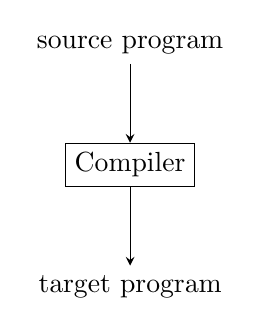
\begin{tikzpicture}[>=stealth]
  % Draw the labelled box. ``compiler'' is its label, and how
  % it is referred to within this TikZ picture. Its displayed
  % text is ``Compiler''. I.e. generically we'd write
  %
  % \node [draw] (nodelabel) {some text};
  %
  \node [draw] (compiler) {Compiler};

  % Create an input node, with the text ``source program'' 
  % which is above the box named ``compiler'', see above.
  \node [above=of compiler] (input) {source program};

  % Create an output node, with the text ``target program'' 
  % which is below the box named ``compiler'', see above.
  \node [below=of compiler] (output) {target program};

  % Draw an arrow _from_ the input node, to the compiler node.
  \draw [->] (input) -- (compiler);

  % Draw an array _from_ the compiler node to the output node.
  \draw [->] (compiler) -- (output);
\end{tikzpicture}

  \caption{A compiler}
  \label{fig:compiler}
\end{figure}

Conversely, a \emph{decompiler} is also a that performs the reverse
operation of a compiler. It too, is a compiler. Commonly one views a
compiler as a translator from a high-level human-readable source
language into a low-level machine-readable language, similarly a
decompiler translates in the opposite direction; see
Fig. \ref{fig:decompiler}. 

The two exhibit a chiral relation to one another, i. e. that they are
mirrored images of each other in terms of functionality, but they are
not themselves identical.

\begin{figure}[H]
  \centering
  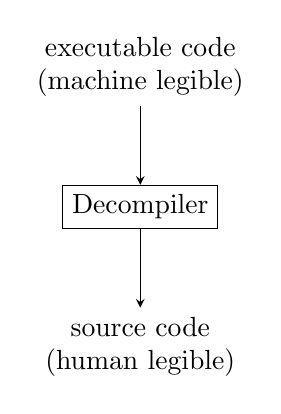
\begin{tikzpicture}[>=stealth]
  \node [draw] (decompiler) {Decompiler};
  \node [above=of decompiler, align=center] (input) {executable code \\ (machine legible)};
  \node [below=of decompiler, align=center] (output) {source code \\ (human legible)};
  \draw [->] (input) -- (decompiler);
  \draw [->] (decompiler) -- (output);
\end{tikzpicture}

  \caption{A decompiler}
  \label{fig:decompiler}
\end{figure}

In this assignment the decompiler must be able to translate from the
machine-readable language of 32-bit numbers representing MIPS32
instructions to the human-readable target language described in the
introduction. See \ref{fig:mipsdecompiler}

\begin{figure}[H]
  \centering
  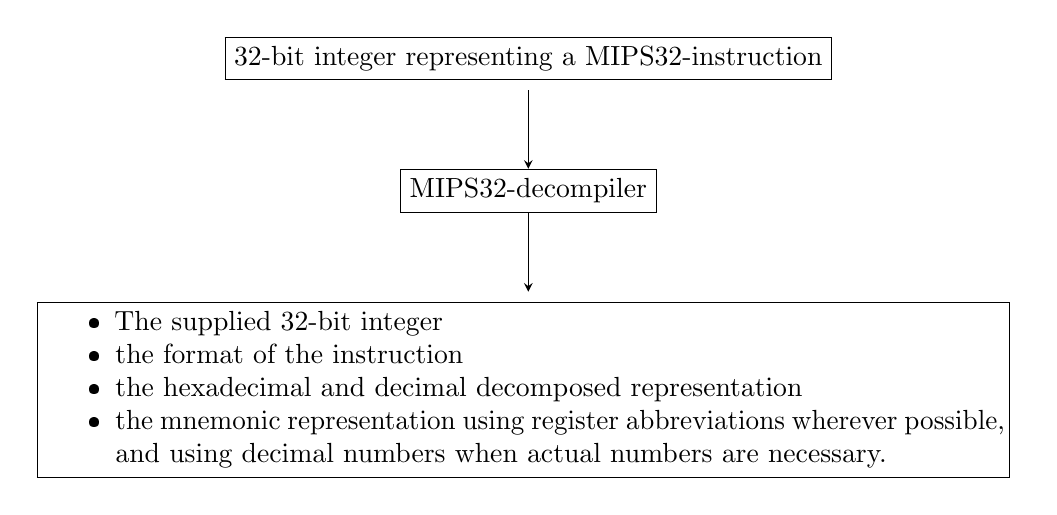
\begin{tikzpicture}[>=stealth]
  \node [draw] (decompiler) {MIPS32-decompiler};
  \node [above=of decompiler, align=center] (input) {\framebox{32-bit integer representing a MIPS32-instruction}};
  \node [below=of decompiler, align=center] (output) {
    \framebox{\begin{varwidth}{\linewidth}\begin{itemize}
          \item The supplied 32-bit integer
          \item the format of the instruction
          \item the hexadecimal and decimal decomposed representation
          \item the mnemonic representation using register
            abbreviations wherever possible, and using decimal numbers
            when actual numbers are necessary.
    \end{itemize}\end{varwidth}}
  };
  \draw [->] (input) -- (decompiler);
  \draw [->] (decompiler) -- (output);
\end{tikzpicture}

  \caption{Our MIPS32-decompiler}
  \label{fig:mipsdecompiler}
\end{figure}

\ref{fig:entrypointdecompiler} describes the programs entry-point into the
decompilation of an instruction.

\begin{figure}[H]
  \centering
  \begin{tikzpicture}[>=stealth]
  \node [draw] (compiler) {\mintinline{java}{Instruction.fromInteger}};
  \node [above=of compiler] (input) {32-bit integer (\mintinline{java}{int})};
  \node [below=of compiler] (output) {\mintinline{java}{Instruction}};
  \draw [->] (input) -- (compiler);
  \draw [->] (compiler) -- (output);
\end{tikzpicture}

  \caption{Entry point for our decompiler}
  \label{fig:entrypointdecompiler}
\end{figure}


% Uses the following files
%
% \subsection{MIPS, RISC and CISC}

MIPS (originally an acronym for Microprocessor without Interlocked
Pipeline Stages) is a ``reduced instruction set computer'' (RISC), as
opposed to a ``complex instruction set computer'' (CISC), instruction
set architecture (ISA) developed by MIPS Technologies (formerly MIPS
Computer Systems, Inc.). Meanwhile, RISC is a [design] concept
developed at IBM, Stanford and UC Berkeley in the late 1970s and early
1980s to overcome the typical deficiencies of CPUs of the 1970s
 \cite{CNS:RISC-Architecture}\cite{Stokes:1999:RISCvsCISC}. Specifically the deficiencies
experienced with CISC ISAs.
% This ending sentence is iffy.

We find that RISC offers two expressly \emph{practical} advantages
over CISC. Per definition RISC has fewer and simpler instructions,
and in 2001 Bart Trzynadlowski showed that the \tt{tst}, \tt{beq},
\tt{bne}, \tt{move}, \tt{cmp}, \tt{cmpi} make up more
than 70\% of all instructions executed on a Motorola
M68K.\footnote{While many associate Motorola with cell-phones, and
  rightfully so, the M68K was a 32-bit CISC microprocessor that were
  used in calculators, UNIX workstations, and the Space Shuttle}
\cite{Trzynadlowski:2001:68k} 

The idea of the ``quantitative approach to computer design''
\cite{Patterson:2008:COD:1502247} is to make the common case fast,
which in itself is one of the four corner-stone design principles
behind RISC.\footnote{The remaining three are ``Simplicity favors
  regularity'', ``Smaller is faster'', and ``Good design demands
  compromises''.\cite{Irwin:CSE331W02.11:2007:PSU}}

A CISC-architecture requires the use of a microcode interpreter but by
removing complex instructions from the instruction set the interpreter
is made obsolete, as decoding is easier. This effect is compounded
further if all of the instructions have the same width. All remaining
instructions can be executed in one clock cycle, which makes
pipelining and superscalar execution ``easy''. The design is a lot
simpler, work has been moved from hardware to software.

\textbf{A load/store architecture and more registers}

As the RISC architecture makes both the microcode interpreter and the
``complex instruction'' decoder redundant we can use the transistors
otherwise occupied by the aforementioned two so that they may be used
for other purposes, for instance multiple ALUs, better pipelining
logic and many additional registers.

A CPU with more registers affords more operations to be performed on
its registers, alleviating the significant cost of memory accesses
resulting in greater performance. With RISC there cannot be any
implicit memory accesses, as there can be in CISC, hence the term
``load/store architecture'': all memory accesses are only possible
through load and store instructions; all other operations only work on
registers.

The time required for a program to execute is calculated using this
formula:

\begin{equation*}
\frac{\textrm{time}}{\textrm{program}} =
\frac{\textrm{time}}{\textrm{cycle}} \cdot
\frac{\textrm{cycles}}{\textrm{instruction}} \cdot
\frac{\textrm{instructions}}{\textrm{program}}
\end{equation*}

CISC CPUs keep the number of instructions per program low, while the
time/cycle is high.  Because RISC CPUs do not have complex
instructions, the number of instructions per program is higher, but
this is compensated by a lower number of cycles per instruction. 

Beyond its practical applications RISC is also well-suited for
academic excursions such as this one. With a smaller set of
instructions, all of equal width, it is arguably better suited as a
pedagogical teaching tool for understanding the internal operation of
a modern microprocessor.

% \subsection{Instruction Encoding}

In the MIPS32 architecture, all machine instructions are represented
as 32-bit numbers. Throughout this document we will intermittently
dissect these 32-bits into various lengths. We regard the ``upper''
--- or equivalently the ``leftmost'' --- bits as the most significant
bits. Hence, we consider the bit order to be little endian.

In little endian bit notation we denote bit 0 as being the least
significant bit (LSB) and bit 31 as the most significant bit (MSB).

Then, for all MIPS32 instructions we have that the leftmost six bits,
31-26, forms the primary opcode. These bits constitute a field which
are referred to as the \tt{op} field of the instruction.
Depending on the value of the primary opcode there can be an extended
opcode in the rightmost six bits, i.e. bits 0 through 5.  These bits
are referred to as the \funct{} field.\footnote{The decoding of
  the \funct{} field provides details of the required operation
  to the \tt{ALU}.}

Ostensibly, the different fields a MIPS instruction should be divided
into is determined solely by the opcode. The manner in which the bits
are divvied up into fields depends on which instruction format that
the instruction has.

Regardless of the type of the instruction we have that the
\opcode{} field is the uppermost six bits of all MIPS
instructions. Opcode, short for ``operation code'', either identifies
a unique instruction or a \emph{set} of instructions.

While MIPS consists of over a 100 different instructions only 6 bits
are used for the \opcode{}, meaning that the
\opcode{}-field can only be used to differentiate between
$2^6=64$ instructions. 

For R-type instructions an additional 6 bits are used (\textbf{B5-0})
called the ``function'', which serves as a secondary opcode to
identify the instruction. I.e. the tuple

\begin{equation*}
(\opcode{},\ \funct{})
\end{equation*}

is sufficient to \emph{uniquely} identify an R-type instruction.

Other instructions, such as \texttt{bltzal}\footnote{Not an R-type
instruction}, is identified by the tuple

\begin{equation*}
(\opcode{}=1,\ \rt{}=16) \textrm{\hspace{1em}(Remark: base 10)}
\end{equation*}

The MIPS ISA groups its instructions into three
categories:\footnote{Some people consider floating-point and branching
  instructions to be their own respective categories} R-type, I-type, and J-type.

\subsubsection{R-type format}

R-type instructions refer to \emph{register} type instructions. These,
when encoded in machine code, are split into 6 fields of lengths 6, 5,
5, 5, 5, 6 respectively, see ~\autoref{fig:r-type-format-bit-fields}.

\begin{figure}[H]
  % Center the image on the page using makebox  
  \makebox[\textwidth][c]{
    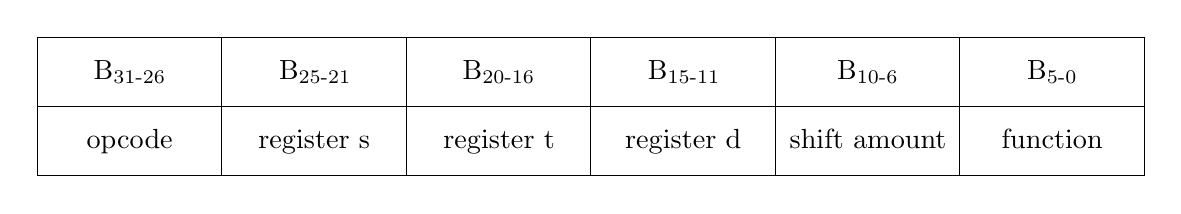
\begin{tikzpicture}[auto,
    every node/.style={rectangle, minimum height=2.5em, text centered, text width=6em, text height=1.5ex, text depth=.25ex},
    field/.style={draw}]
\matrix (m) [ampersand replacement=\&, column sep=-\pgflinewidth, row sep=-\pgflinewidth]
{
\node [field] {$\textrm{B}_{31\textrm{-}26}$}; \&
\node [field] {$\textrm{B}_{25\textrm{-}21}$}; \&
\node [field] {$\textrm{B}_{20\textrm{-}16}$}; \&
\node [field] {$\textrm{B}_{15\textrm{-}11}$}; \&
\node [field] {$\textrm{B}_{10\textrm{-}6}$}; \&
\node [field] {$\textrm{B}_{5\textrm{-}0}$}; \&
\\
\node [field] {opcode}; \&
\node [field] {register s}; \&
\node [field] {register t}; \&
\node [field] {register d}; \&
\node [field] {shift amount}; \&
\node [field] {function}; \&
\\
};
\end{tikzpicture}
%
  } 
  \caption{The bitfields of an R-type format instruction}
  \label{fig:r-type-format-bit-fields}
\end{figure}

For instance, \tt{add} is an R-type instruction, and in
its mnemonic form it looks like

\begin{lstlisting}[style=mips_lst]
add $rd, $rs, $rt
\end{lstlisting}
%$

where \tt{\$rd} refers to some register \tt{d}.

The semantics of the instruction is

\begin{lstlisting}[style=semantics_lst]
R[d] = R[s] + R[t]
\end{lstlisting}

where the addition is signed addition. Hence, \tt{\$rd} is the
target/destination register while the operands \tt{\$rs} and
\tt{\$rt} are the two source registers.\footnote{Notice that the
  mnemonic representation specifies the destination register
  \emph{first} followed by the two source registers but the the actual
  binary format stores the two source registers first, then the
  destination register.}

Certain R-type instructions places certain constraints on its
constituent fields beyond the value of the opcode and the funct
field. Several instructions are only valid if \shamt{} is set to
0, and specifies the shift amount used by shifting instructions such
as \tt{sll} (shift left logical). \tt{clo} (count leading
zeroes) expects both \shamt{} and \tt{rt} to be equal to
zero, and meanwhile \tt{div} (divide with overflow) expects
\rd{} and \shamt{} to be zero.

\subsubsection{I-type format}

I-type stands for "immediate type", and it is decomposed into four
fields. See ~\autoref{fig:i-type-format-bit-fields}.

\begin{figure}[H]
  \makebox[\textwidth][c]{
    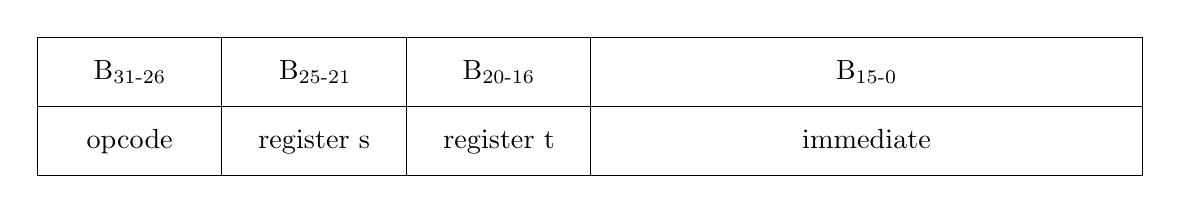
\begin{tikzpicture}[auto,
    every node/.style={rectangle, minimum height=2.5em, text centered, text width=6em, text height=1.5ex, text depth=.25ex},
    field/.style={draw, anchor=west}]
\matrix (m) [ampersand replacement=\&, column sep=-\pgflinewidth, row sep=-\pgflinewidth]
{
\node [field] {$\textrm{B}_{31\textrm{-}26}$}; \&
\node [field] {$\textrm{B}_{25\textrm{-}21}$}; \&
\node [field] {$\textrm{B}_{20\textrm{-}16}$}; \&
\node [field, text width=19.25em] {$\textrm{B}_{15\textrm{-}0}$}; \&
\\
\node [field] {opcode}; \&
\node [field] {register s}; \&
\node [field] {register t}; \&
\node [field, text width=19.25em] {immediate}; \&
\\
};
\end{tikzpicture}
%
  }
  \caption{The bitfields of an I-type format instruction}
  \label{fig:i-type-format-bit-fields}
\end{figure}

The prototypical I-type instruction in its mnemonic form looks as follows,

\begin{lstlisting}[style=mips_lst]
addi $rt, $rs, immed
\end{lstlisting}

In this case, \tt{\$rt} is the destination register, and
\tt{\$rs} is the \emph{only} source register.

The semantics of the \tt{addi} instruction is

\begin{lstlisting}[style=semantics_lst]
R[t] = R[s] + (IR$_{15})^{16}$ IR$_{15\textrm{-}0}$
\end{lstlisting}

where \tt{IR} refers to the instruction register, the register
where the current instruction is stored. \tt{(IR$_{15}$)$^{16}$}
means that bit \textbf{B15} of the instruction register (which is the
sign bit of the immediate value) is repeated 16 times. This is then
followed by \tt{IR$_{15\textrm{-}0}$}, which is the 16 bits of
the immediate value.

Basically, the semantics says to sign-extend the immediate value to 32
bits, add it (using signed addition) to register \tt{R[s]}, and store
the result in register \tt{\$rt}.

For an example,

\begin{lstlisting}[style=mips_lst]
addi $s1, $s2, 100
\end{lstlisting}
%$

stores the value of $(\tt{\$s2} + 100)$ in \tt{\$s1}.

\subsubsection{J-type format}

All jump instructions belong to the J-type format

J-type instructions refer to \emph{jump} type instructions. These,
when encoded in machine code, are split into 2 fields of lengths 6 and
26, respectively. See ~\autoref{fig:r-type-format-bit-fields}.

\begin{figure}[H]
  \makebox[\textwidth][c]{
    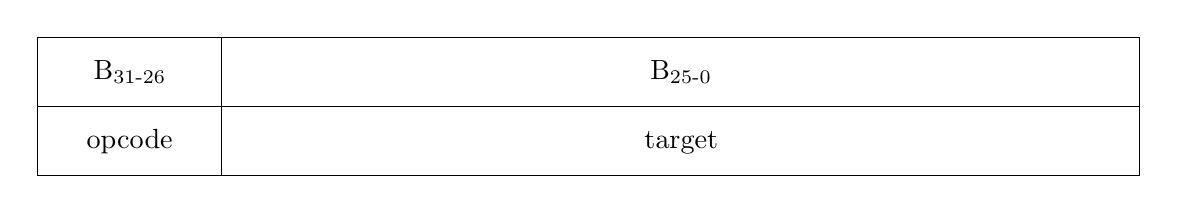
\begin{tikzpicture}[auto,
    every node/.style={rectangle, minimum height=2.5em, text centered, text width=6em, text height=1.5ex, text depth=.25ex},
    field/.style={draw}]
\matrix (m) [ampersand replacement=\&, column sep=-\pgflinewidth, row sep=-\pgflinewidth]
{
\node [field] {$\textrm{B}_{31\textrm{-}26}$}; \&
\node [field, text width=32.5 em] {$\textrm{B}_{25\textrm{-}0}$}; \&
\\
\node [field] {opcode}; \&
\node [field, text width=32.5 em] {target}; \&
\\
};
\end{tikzpicture}
%
  }
  \caption{The bitfields of an J-type format instruction}
  \label{fig:j-type-format-bit-fields}
\end{figure}

For an example the instruction \tt{j} is J-type instruction, and in
its mnemonic form as follows,

\begin{lstlisting}[style=mips_lst]
j target
\end{lstlisting}
%$

\tt{j} is the archetypal jump instruction. In ~\autoref{lst:jump}
``\PC{}'' stands for ``program counter''. The program counter stores
the current address of the instruction that is \emph{currently}
being executed.

In effect, what the \tt{j} instruction does, as shown in
~\autoref{lst:jump}, is re-assign the \PC{} the 32-bit address given
by the upper 4 bits of the \PC{} followed by the 26-bits making up the
target, followed by two zeroes.

\begin{lstlisting}[style=semantics_lst, label={lst:jump}]
PC := PC$_{31\textrm{-}28}$ IR$_{25\textrm{-}0}$ 00
\end{lstlisting}


% \subsubsection{MIPS Register Naming and Usage Convention}

Within the MIPS32 architecture there are 32 general-purpose registers,
see \autoref{table:mips-register-naming-and-usage-convention}. The
registers when written out, are preceded by a ``\tt{\$}''.  We use
two formats for addressing a particular register, e.g. \tt{\$0}
through \tt{\$31}. Or, using their equivalent mnemonic
representations, for instance \tt{\$t1}. Both formats may be used
interchangeably in the assembly language.

\begin{table}[H]
\centering
\begin{tabular}{lll}
\toprule
Mnemonic & Register Number & Usage                                                     \\
\midrule
\tt{\$zero}                & 0       & constant 0                                      \\
\tt{\$at}                  & 1       & reserved for assembler                          \\
\tt{\$v0} - \tt{\$v1}      & 2 - 3   & expression evaluation and results of a function \\
\tt{\$a0} - \tt{\$a3}      & 4 - 7   & argument 1 through 4                            \\
\tt{\$t0} - \tt{\$t7}      & 8 - 15  & temporary (not preserved across call)           \\
\tt{\$s0} - \tt{\$s7}      & 16 - 23 & saved temporary (preserved across call          \\
\tt{\$t8} - \tt{\$t9}      & 24 - 25 & temporary (not preserved across call)           \\
\tt{\$k0} - \tt{\$k1}      & 26 - 27 & reserved for OS kernel                          \\
\tt{\$gp}                  & 28      & pointer to global area                          \\
\tt{\$sp}                  & 29      & stack pointer                                   \\
\tt{\$fp}                  & 30      & frame pointer                                   \\
\tt{\$ra}                  & 31      & return address (used by function call)          \\
\bottomrule
\end{tabular}
\caption{MIPS register naming and usage convention}
\label{table:mips-register-naming-and-usage-convention}
\end{table}

% \subsection{Instruction Encoding}

In the MIPS32 architecture, all machine instructions are represented
as 32-bit numbers. Throughout this document we will intermittently
dissect these 32-bits into various lengths. We regard the ``upper''
--- or equivalently the ``leftmost'' --- bits as the most significant
bits. Hence, we consider the bit order to be little endian.

In little endian bit notation we denote bit 0 as being the least
significant bit (LSB) and bit 31 as the most significant bit (MSB).

Then, for all MIPS32 instructions we have that the leftmost six bits,
31-26, forms the primary opcode. These bits constitute a field which
are referred to as the \tt{op} field of the instruction.
Depending on the value of the primary opcode there can be an extended
opcode in the rightmost six bits, i.e. bits 0 through 5.  These bits
are referred to as the \funct{} field.\footnote{The decoding of
  the \funct{} field provides details of the required operation
  to the \tt{ALU}.}

Ostensibly, the different fields a MIPS instruction should be divided
into is determined solely by the opcode. The manner in which the bits
are divvied up into fields depends on which instruction format that
the instruction has.

Regardless of the type of the instruction we have that the
\opcode{} field is the uppermost six bits of all MIPS
instructions. Opcode, short for ``operation code'', either identifies
a unique instruction or a \emph{set} of instructions.

While MIPS consists of over a 100 different instructions only 6 bits
are used for the \opcode{}, meaning that the
\opcode{}-field can only be used to differentiate between
$2^6=64$ instructions. 

For R-type instructions an additional 6 bits are used (\textbf{B5-0})
called the ``function'', which serves as a secondary opcode to
identify the instruction. I.e. the tuple

\begin{equation*}
(\opcode{},\ \funct{})
\end{equation*}

is sufficient to \emph{uniquely} identify an R-type instruction.

Other instructions, such as \texttt{bltzal}\footnote{Not an R-type
instruction}, is identified by the tuple

\begin{equation*}
(\opcode{}=1,\ \rt{}=16) \textrm{\hspace{1em}(Remark: base 10)}
\end{equation*}

The MIPS ISA groups its instructions into three
categories:\footnote{Some people consider floating-point and branching
  instructions to be their own respective categories} R-type, I-type, and J-type.

\subsubsection{R-type format}

R-type instructions refer to \emph{register} type instructions. These,
when encoded in machine code, are split into 6 fields of lengths 6, 5,
5, 5, 5, 6 respectively, see ~\autoref{fig:r-type-format-bit-fields}.

\begin{figure}[H]
  % Center the image on the page using makebox  
  \makebox[\textwidth][c]{
    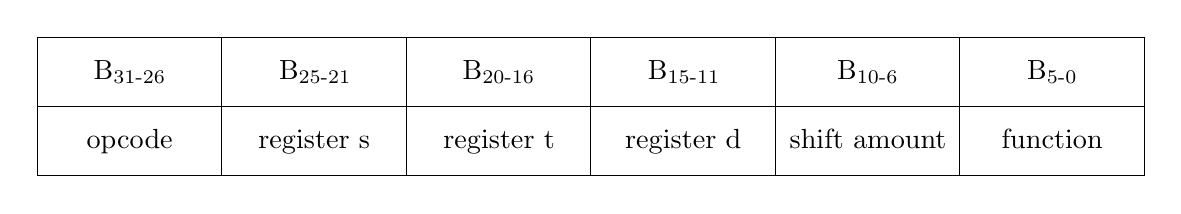
\begin{tikzpicture}[auto,
    every node/.style={rectangle, minimum height=2.5em, text centered, text width=6em, text height=1.5ex, text depth=.25ex},
    field/.style={draw}]
\matrix (m) [ampersand replacement=\&, column sep=-\pgflinewidth, row sep=-\pgflinewidth]
{
\node [field] {$\textrm{B}_{31\textrm{-}26}$}; \&
\node [field] {$\textrm{B}_{25\textrm{-}21}$}; \&
\node [field] {$\textrm{B}_{20\textrm{-}16}$}; \&
\node [field] {$\textrm{B}_{15\textrm{-}11}$}; \&
\node [field] {$\textrm{B}_{10\textrm{-}6}$}; \&
\node [field] {$\textrm{B}_{5\textrm{-}0}$}; \&
\\
\node [field] {opcode}; \&
\node [field] {register s}; \&
\node [field] {register t}; \&
\node [field] {register d}; \&
\node [field] {shift amount}; \&
\node [field] {function}; \&
\\
};
\end{tikzpicture}
%
  } 
  \caption{The bitfields of an R-type format instruction}
  \label{fig:r-type-format-bit-fields}
\end{figure}

For instance, \tt{add} is an R-type instruction, and in
its mnemonic form it looks like

\begin{lstlisting}[style=mips_lst]
add $rd, $rs, $rt
\end{lstlisting}
%$

where \tt{\$rd} refers to some register \tt{d}.

The semantics of the instruction is

\begin{lstlisting}[style=semantics_lst]
R[d] = R[s] + R[t]
\end{lstlisting}

where the addition is signed addition. Hence, \tt{\$rd} is the
target/destination register while the operands \tt{\$rs} and
\tt{\$rt} are the two source registers.\footnote{Notice that the
  mnemonic representation specifies the destination register
  \emph{first} followed by the two source registers but the the actual
  binary format stores the two source registers first, then the
  destination register.}

Certain R-type instructions places certain constraints on its
constituent fields beyond the value of the opcode and the funct
field. Several instructions are only valid if \shamt{} is set to
0, and specifies the shift amount used by shifting instructions such
as \tt{sll} (shift left logical). \tt{clo} (count leading
zeroes) expects both \shamt{} and \tt{rt} to be equal to
zero, and meanwhile \tt{div} (divide with overflow) expects
\rd{} and \shamt{} to be zero.

\subsubsection{I-type format}

I-type stands for "immediate type", and it is decomposed into four
fields. See ~\autoref{fig:i-type-format-bit-fields}.

\begin{figure}[H]
  \makebox[\textwidth][c]{
    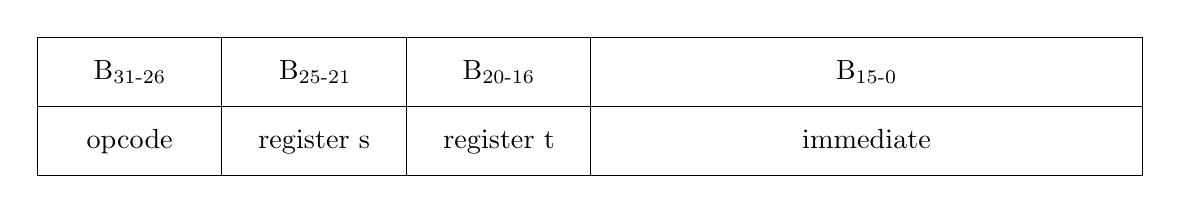
\begin{tikzpicture}[auto,
    every node/.style={rectangle, minimum height=2.5em, text centered, text width=6em, text height=1.5ex, text depth=.25ex},
    field/.style={draw, anchor=west}]
\matrix (m) [ampersand replacement=\&, column sep=-\pgflinewidth, row sep=-\pgflinewidth]
{
\node [field] {$\textrm{B}_{31\textrm{-}26}$}; \&
\node [field] {$\textrm{B}_{25\textrm{-}21}$}; \&
\node [field] {$\textrm{B}_{20\textrm{-}16}$}; \&
\node [field, text width=19.25em] {$\textrm{B}_{15\textrm{-}0}$}; \&
\\
\node [field] {opcode}; \&
\node [field] {register s}; \&
\node [field] {register t}; \&
\node [field, text width=19.25em] {immediate}; \&
\\
};
\end{tikzpicture}
%
  }
  \caption{The bitfields of an I-type format instruction}
  \label{fig:i-type-format-bit-fields}
\end{figure}

The prototypical I-type instruction in its mnemonic form looks as follows,

\begin{lstlisting}[style=mips_lst]
addi $rt, $rs, immed
\end{lstlisting}

In this case, \tt{\$rt} is the destination register, and
\tt{\$rs} is the \emph{only} source register.

The semantics of the \tt{addi} instruction is

\begin{lstlisting}[style=semantics_lst]
R[t] = R[s] + (IR$_{15})^{16}$ IR$_{15\textrm{-}0}$
\end{lstlisting}

where \tt{IR} refers to the instruction register, the register
where the current instruction is stored. \tt{(IR$_{15}$)$^{16}$}
means that bit \textbf{B15} of the instruction register (which is the
sign bit of the immediate value) is repeated 16 times. This is then
followed by \tt{IR$_{15\textrm{-}0}$}, which is the 16 bits of
the immediate value.

Basically, the semantics says to sign-extend the immediate value to 32
bits, add it (using signed addition) to register \tt{R[s]}, and store
the result in register \tt{\$rt}.

For an example,

\begin{lstlisting}[style=mips_lst]
addi $s1, $s2, 100
\end{lstlisting}
%$

stores the value of $(\tt{\$s2} + 100)$ in \tt{\$s1}.

\subsubsection{J-type format}

All jump instructions belong to the J-type format

J-type instructions refer to \emph{jump} type instructions. These,
when encoded in machine code, are split into 2 fields of lengths 6 and
26, respectively. See ~\autoref{fig:r-type-format-bit-fields}.

\begin{figure}[H]
  \makebox[\textwidth][c]{
    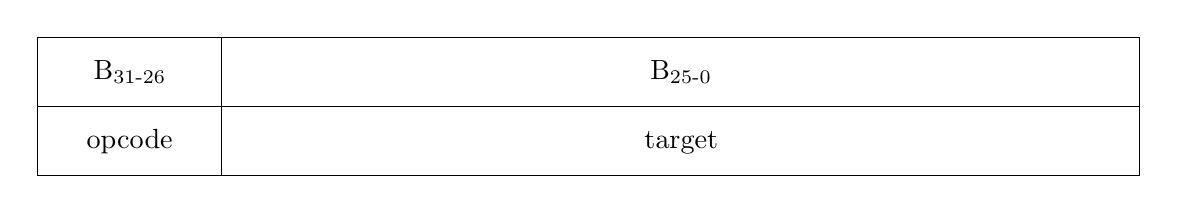
\begin{tikzpicture}[auto,
    every node/.style={rectangle, minimum height=2.5em, text centered, text width=6em, text height=1.5ex, text depth=.25ex},
    field/.style={draw}]
\matrix (m) [ampersand replacement=\&, column sep=-\pgflinewidth, row sep=-\pgflinewidth]
{
\node [field] {$\textrm{B}_{31\textrm{-}26}$}; \&
\node [field, text width=32.5 em] {$\textrm{B}_{25\textrm{-}0}$}; \&
\\
\node [field] {opcode}; \&
\node [field, text width=32.5 em] {target}; \&
\\
};
\end{tikzpicture}
%
  }
  \caption{The bitfields of an J-type format instruction}
  \label{fig:j-type-format-bit-fields}
\end{figure}

For an example the instruction \tt{j} is J-type instruction, and in
its mnemonic form as follows,

\begin{lstlisting}[style=mips_lst]
j target
\end{lstlisting}
%$

\tt{j} is the archetypal jump instruction. In ~\autoref{lst:jump}
``\PC{}'' stands for ``program counter''. The program counter stores
the current address of the instruction that is \emph{currently}
being executed.

In effect, what the \tt{j} instruction does, as shown in
~\autoref{lst:jump}, is re-assign the \PC{} the 32-bit address given
by the upper 4 bits of the \PC{} followed by the 26-bits making up the
target, followed by two zeroes.

\begin{lstlisting}[style=semantics_lst, label={lst:jump}]
PC := PC$_{31\textrm{-}28}$ IR$_{25\textrm{-}0}$ 00
\end{lstlisting}


% \subsubsection{Example: Numeric decoding}

Consider the machine-language MIPS32 instruction \tt{0x71014802}.
Depending on the format of the instruction it decomposes into fields
varying lengths.

Recall that for all numbers in the MIPS32 instruction set the leftmost
six bits always represent the opcode for the instruction. The opcode
alone is not always sufficient to identify the particular instruction,
\emph{but} it is always sufficient to identify the format of the
instruction.

The leftmost six bits of \tt{0x71014802} is \tt{0x1c}. It is
\emph{known} that this number corresponds to a set of instructions in
the R-type format. The format specifies into which fields the 32-bit
decomposes into. The number of bits composing each respective field is
given in the bottom row of ~\autoref{fig:r-decomposed},

\begin{figure}[H]
\centering
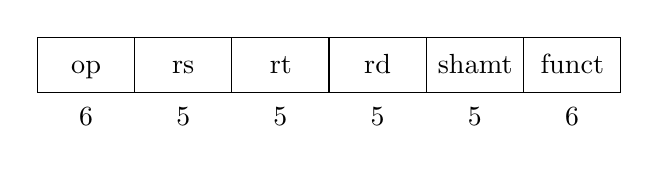
\begin{tikzpicture}[node distance=1em]

\matrix (decomposed-representation) [
  matrix of nodes,
  row sep=0.2em,
  column sep=-\pgflinewidth,
  row 1/.style={
    nodes={
      rectangle, 
      draw, 
      text centered,
          text width=10mm,
      anchor=base,
      text height=.8em,text depth=.2em,minimum size=7mm
    }
  }
] {
op & rs & rt & rd & shamt & funct \\
6 & 5 & 5 & 5 & 5 & 6 \\
};
\end{tikzpicture}

\caption{The length of each respective field for R-type format instructions}
\label{fig:r-decomposed}
\end{figure}

Decomposing \tt{0x71014802} into the fields shown in
\autoref{fig:r-decomposed} yields \tt{rs=8}, \tt{rt=1}, \tt{rd=9},
\tt{shamt=0}, and \tt{funct=2}. The \emph{decomposed representation}
of this instruction in hexadecimal form is thus \tt{[0x1c 8 1 9 0
  2]}.\footnote{The corresponding \emph{decimal representation} is
  \tt{[28 8 1 9 0 2]}}

To identify the particular instruction represented by \tt{0x71014802}
the \funct{} field must be consulted. Pairing the opcode, \tt{0x1c}
and the value in the \funct{} field uniquely identifies the
instruction a \tt{mul} instruction; see \autoref{fig:mul-decomposed}.

\begin{figure}[H]
  \centering
  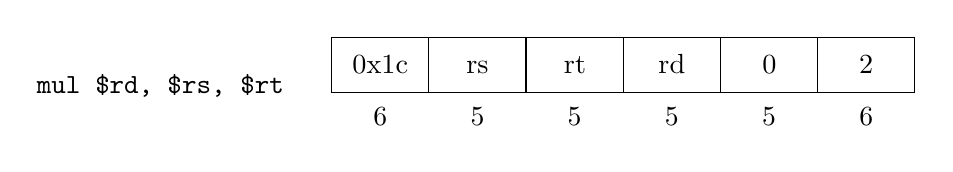
\begin{tikzpicture}[node distance=1em]
\matrix (decomposed-representation) [
  matrix of nodes,
  row sep=0.2em,
  column sep=-\pgflinewidth,
  row 1/.style={
    nodes={
      rectangle, 
      draw, 
      text centered,
          text width=10mm,
      anchor=base,
      text height=.8em,text depth=.2em,minimum size=7mm
    }
  }
] {
0x1c & rs & rt & rd & 0 & 2 \\
6 & 5 & 5 & 5 & 5 & 6 \\
};
\node [left=of decomposed-representation] (mnemonic-representation) {\texttt{mul \$rd, \$rs, \$rt}};
\end{tikzpicture}

  \caption{Decomposition and mnemonic representation of \tt{mul}}
  \label{fig:mul-decomposed}
\end{figure}

Earlier we determined the fields \tt{rs}, \tt{rt} and \rd{} to have
the addresses 8, 1, and 9, respectively. In MIPS registers are named,
following the convention shown in
\autoref{table:mips-register-naming-and-usage-convention}

Replacing the numerical values of \tt{rs}, \tt{rt} and \rd{}, with
their named counterparts yields the \emph{mnemonic representation} of
the instruction to be

\begin{lstlisting}[style=mips_lst]
mul $t1, $t0, $at
\end{lstlisting}
%$

% \subsubsection{Example: Mnemonic decoding}

The reverse operation, translating from a human-legible form to the
numerical form, is trivial. Given, of course, that you know the format
that the mnemonic form is in and any conditions pertaining to the
particular instruction. 

Take for instance \tt{div \$t2, \$t4}, given that we know its mnemonic
representation to be on the form

\begin{lstlisting}[style=mips_lst]
div $rs, $rt
\end{lstlisting}
%$

and that due to its nature both \shamt{} and \rd{} is both zero,
together with the fact that we know its opcode and \funct{}, trivially
we substitute all those values in together with the register
addresses. Together we get

\begin{figure}[H]
  \makebox[\textwidth][c]{
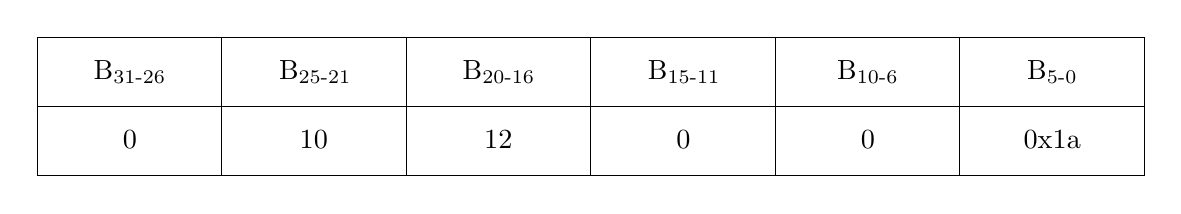
\begin{tikzpicture}[auto,
    every node/.style={rectangle, minimum height=2.5em, text centered, text width=6em, text height=1.5ex, text depth=.25ex},
    field/.style={draw}]
\matrix (m) [ampersand replacement=\&, column sep=-\pgflinewidth, row sep=-\pgflinewidth]
{
\node [field] {$\textrm{B}_{31\textrm{-}26}$}; \&
\node [field] {$\textrm{B}_{25\textrm{-}21}$}; \&
\node [field] {$\textrm{B}_{20\textrm{-}16}$}; \&
\node [field] {$\textrm{B}_{15\textrm{-}11}$}; \&
\node [field] {$\textrm{B}_{10\textrm{-}6}$}; \&
\node [field] {$\textrm{B}_{5\textrm{-}0}$}; \&
\\
\node [field] {0}; \&
\node [field] {10}; \&
\node [field] {12}; \&
\node [field] {0}; \&
\node [field] {0}; \&
\node [field] {0x1a}; \&
\\
};
\end{tikzpicture}
  }
\end{figure}

and the final translation step, and the resulting numerical
representation, is given by a sequence of bit-shift operations, in
this case the following will serve,\footnote{No operations are
  required for the zeroes.}\footnote{Notice that the shift amount (21,
  16) corresponds directly to the lower most bit of the respective fields (rs, rt)}

\begin{lstlisting}
(10 << 21) | (12 << 16) | 0x1a
\end{lstlisting}

which is equal to \tt{0x014c001a}.

%
% Mentioned for reference so one can see if any section is missing
\section{Technical background}

In this section we will introduce MIPS, juxtapose the two instruction
set architectures RISC and CISC, and provide a cursory overview --- as
well as reviewing (briefly) --- the MIPS instruction set in
preparation for the rest of this document.

\subsection{MIPS, RISC and CISC}

MIPS (originally an acronym for Microprocessor without Interlocked
Pipeline Stages) is a ``reduced instruction set computer'' (RISC), as
opposed to a ``complex instruction set computer'' (CISC), instruction
set architecture (ISA) developed by MIPS Technologies (formerly MIPS
Computer Systems, Inc.). Meanwhile, RISC is a [design] concept
developed at IBM, Stanford and UC Berkeley in the late 1970s and early
1980s to overcome the typical deficiencies of CPUs of the 1970s
 \cite{CNS:RISC-Architecture}\cite{Stokes:1999:RISCvsCISC}. Specifically the deficiencies
experienced with CISC ISAs.
% This ending sentence is iffy.

We find that RISC offers two expressly \emph{practical} advantages
over CISC. Per definition RISC has fewer and simpler instructions,
and in 2001 Bart Trzynadlowski showed that the \tt{tst}, \tt{beq},
\tt{bne}, \tt{move}, \tt{cmp}, \tt{cmpi} make up more
than 70\% of all instructions executed on a Motorola
M68K.\footnote{While many associate Motorola with cell-phones, and
  rightfully so, the M68K was a 32-bit CISC microprocessor that were
  used in calculators, UNIX workstations, and the Space Shuttle}
\cite{Trzynadlowski:2001:68k} 

The idea of the ``quantitative approach to computer design''
\cite{Patterson:2008:COD:1502247} is to make the common case fast,
which in itself is one of the four corner-stone design principles
behind RISC.\footnote{The remaining three are ``Simplicity favors
  regularity'', ``Smaller is faster'', and ``Good design demands
  compromises''.\cite{Irwin:CSE331W02.11:2007:PSU}}

A CISC-architecture requires the use of a microcode interpreter but by
removing complex instructions from the instruction set the interpreter
is made obsolete, as decoding is easier. This effect is compounded
further if all of the instructions have the same width. All remaining
instructions can be executed in one clock cycle, which makes
pipelining and superscalar execution ``easy''. The design is a lot
simpler, work has been moved from hardware to software.

\textbf{A load/store architecture and more registers}

As the RISC architecture makes both the microcode interpreter and the
``complex instruction'' decoder redundant we can use the transistors
otherwise occupied by the aforementioned two so that they may be used
for other purposes, for instance multiple ALUs, better pipelining
logic and many additional registers.

A CPU with more registers affords more operations to be performed on
its registers, alleviating the significant cost of memory accesses
resulting in greater performance. With RISC there cannot be any
implicit memory accesses, as there can be in CISC, hence the term
``load/store architecture'': all memory accesses are only possible
through load and store instructions; all other operations only work on
registers.

The time required for a program to execute is calculated using this
formula:

\begin{equation*}
\frac{\textrm{time}}{\textrm{program}} =
\frac{\textrm{time}}{\textrm{cycle}} \cdot
\frac{\textrm{cycles}}{\textrm{instruction}} \cdot
\frac{\textrm{instructions}}{\textrm{program}}
\end{equation*}

CISC CPUs keep the number of instructions per program low, while the
time/cycle is high.  Because RISC CPUs do not have complex
instructions, the number of instructions per program is higher, but
this is compensated by a lower number of cycles per instruction. 

Beyond its practical applications RISC is also well-suited for
academic excursions such as this one. With a smaller set of
instructions, all of equal width, it is arguably better suited as a
pedagogical teaching tool for understanding the internal operation of
a modern microprocessor.

\subsection{Instruction Encoding}

In the MIPS32 architecture, all machine instructions are represented
as 32-bit numbers. Throughout this document we will intermittently
dissect these 32-bits into various lengths. We regard the ``upper''
--- or equivalently the ``leftmost'' --- bits as the most significant
bits. Hence, we consider the bit order to be little endian.

In little endian bit notation we denote bit 0 as being the least
significant bit (LSB) and bit 31 as the most significant bit (MSB).

Then, for all MIPS32 instructions we have that the leftmost six bits,
31-26, forms the primary opcode. These bits constitute a field which
are referred to as the \tt{op} field of the instruction.
Depending on the value of the primary opcode there can be an extended
opcode in the rightmost six bits, i.e. bits 0 through 5.  These bits
are referred to as the \funct{} field.\footnote{The decoding of
  the \funct{} field provides details of the required operation
  to the \tt{ALU}.}

Ostensibly, the different fields a MIPS instruction should be divided
into is determined solely by the opcode. The manner in which the bits
are divvied up into fields depends on which instruction format that
the instruction has.

Regardless of the type of the instruction we have that the
\opcode{} field is the uppermost six bits of all MIPS
instructions. Opcode, short for ``operation code'', either identifies
a unique instruction or a \emph{set} of instructions.

While MIPS consists of over a 100 different instructions only 6 bits
are used for the \opcode{}, meaning that the
\opcode{}-field can only be used to differentiate between
$2^6=64$ instructions. 

For R-type instructions an additional 6 bits are used (\textbf{B5-0})
called the ``function'', which serves as a secondary opcode to
identify the instruction. I.e. the tuple

\begin{equation*}
(\opcode{},\ \funct{})
\end{equation*}

is sufficient to \emph{uniquely} identify an R-type instruction.

Other instructions, such as \texttt{bltzal}\footnote{Not an R-type
instruction}, is identified by the tuple

\begin{equation*}
(\opcode{}=1,\ \rt{}=16) \textrm{\hspace{1em}(Remark: base 10)}
\end{equation*}

The MIPS ISA groups its instructions into three
categories:\footnote{Some people consider floating-point and branching
  instructions to be their own respective categories} R-type, I-type, and J-type.

\subsubsection{R-type format}

R-type instructions refer to \emph{register} type instructions. These,
when encoded in machine code, are split into 6 fields of lengths 6, 5,
5, 5, 5, 6 respectively, see ~\autoref{fig:r-type-format-bit-fields}.

\begin{figure}[H]
  % Center the image on the page using makebox  
  \makebox[\textwidth][c]{
    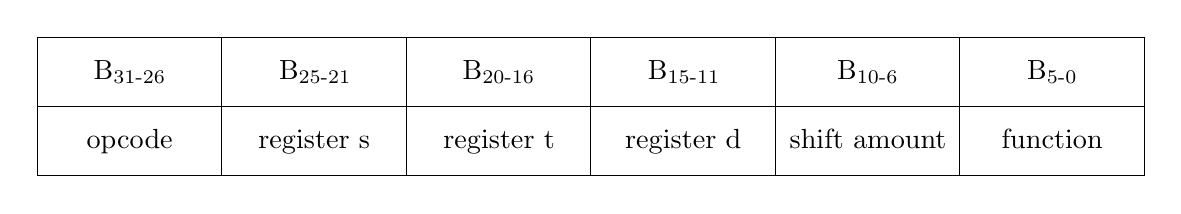
\begin{tikzpicture}[auto,
    every node/.style={rectangle, minimum height=2.5em, text centered, text width=6em, text height=1.5ex, text depth=.25ex},
    field/.style={draw}]
\matrix (m) [ampersand replacement=\&, column sep=-\pgflinewidth, row sep=-\pgflinewidth]
{
\node [field] {$\textrm{B}_{31\textrm{-}26}$}; \&
\node [field] {$\textrm{B}_{25\textrm{-}21}$}; \&
\node [field] {$\textrm{B}_{20\textrm{-}16}$}; \&
\node [field] {$\textrm{B}_{15\textrm{-}11}$}; \&
\node [field] {$\textrm{B}_{10\textrm{-}6}$}; \&
\node [field] {$\textrm{B}_{5\textrm{-}0}$}; \&
\\
\node [field] {opcode}; \&
\node [field] {register s}; \&
\node [field] {register t}; \&
\node [field] {register d}; \&
\node [field] {shift amount}; \&
\node [field] {function}; \&
\\
};
\end{tikzpicture}
%
  } 
  \caption{The bitfields of an R-type format instruction}
  \label{fig:r-type-format-bit-fields}
\end{figure}

For instance, \tt{add} is an R-type instruction, and in
its mnemonic form it looks like

\begin{lstlisting}[style=mips_lst]
add $rd, $rs, $rt
\end{lstlisting}
%$

where \tt{\$rd} refers to some register \tt{d}.

The semantics of the instruction is

\begin{lstlisting}[style=semantics_lst]
R[d] = R[s] + R[t]
\end{lstlisting}

where the addition is signed addition. Hence, \tt{\$rd} is the
target/destination register while the operands \tt{\$rs} and
\tt{\$rt} are the two source registers.\footnote{Notice that the
  mnemonic representation specifies the destination register
  \emph{first} followed by the two source registers but the the actual
  binary format stores the two source registers first, then the
  destination register.}

Certain R-type instructions places certain constraints on its
constituent fields beyond the value of the opcode and the funct
field. Several instructions are only valid if \shamt{} is set to
0, and specifies the shift amount used by shifting instructions such
as \tt{sll} (shift left logical). \tt{clo} (count leading
zeroes) expects both \shamt{} and \tt{rt} to be equal to
zero, and meanwhile \tt{div} (divide with overflow) expects
\rd{} and \shamt{} to be zero.

\subsubsection{I-type format}

I-type stands for "immediate type", and it is decomposed into four
fields. See ~\autoref{fig:i-type-format-bit-fields}.

\begin{figure}[H]
  \makebox[\textwidth][c]{
    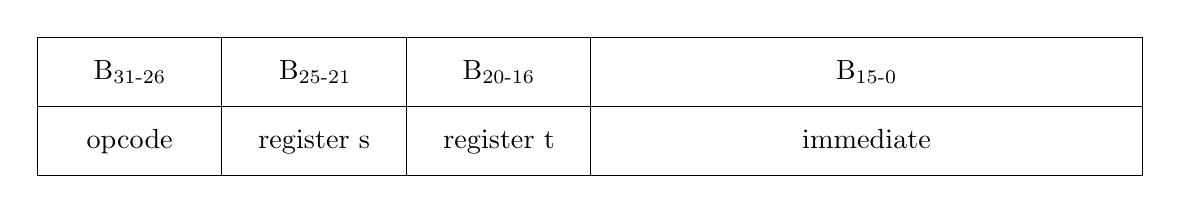
\begin{tikzpicture}[auto,
    every node/.style={rectangle, minimum height=2.5em, text centered, text width=6em, text height=1.5ex, text depth=.25ex},
    field/.style={draw, anchor=west}]
\matrix (m) [ampersand replacement=\&, column sep=-\pgflinewidth, row sep=-\pgflinewidth]
{
\node [field] {$\textrm{B}_{31\textrm{-}26}$}; \&
\node [field] {$\textrm{B}_{25\textrm{-}21}$}; \&
\node [field] {$\textrm{B}_{20\textrm{-}16}$}; \&
\node [field, text width=19.25em] {$\textrm{B}_{15\textrm{-}0}$}; \&
\\
\node [field] {opcode}; \&
\node [field] {register s}; \&
\node [field] {register t}; \&
\node [field, text width=19.25em] {immediate}; \&
\\
};
\end{tikzpicture}
%
  }
  \caption{The bitfields of an I-type format instruction}
  \label{fig:i-type-format-bit-fields}
\end{figure}

The prototypical I-type instruction in its mnemonic form looks as follows,

\begin{lstlisting}[style=mips_lst]
addi $rt, $rs, immed
\end{lstlisting}

In this case, \tt{\$rt} is the destination register, and
\tt{\$rs} is the \emph{only} source register.

The semantics of the \tt{addi} instruction is

\begin{lstlisting}[style=semantics_lst]
R[t] = R[s] + (IR$_{15})^{16}$ IR$_{15\textrm{-}0}$
\end{lstlisting}

where \tt{IR} refers to the instruction register, the register
where the current instruction is stored. \tt{(IR$_{15}$)$^{16}$}
means that bit \textbf{B15} of the instruction register (which is the
sign bit of the immediate value) is repeated 16 times. This is then
followed by \tt{IR$_{15\textrm{-}0}$}, which is the 16 bits of
the immediate value.

Basically, the semantics says to sign-extend the immediate value to 32
bits, add it (using signed addition) to register \tt{R[s]}, and store
the result in register \tt{\$rt}.

For an example,

\begin{lstlisting}[style=mips_lst]
addi $s1, $s2, 100
\end{lstlisting}
%$

stores the value of $(\tt{\$s2} + 100)$ in \tt{\$s1}.

\subsubsection{J-type format}

All jump instructions belong to the J-type format

J-type instructions refer to \emph{jump} type instructions. These,
when encoded in machine code, are split into 2 fields of lengths 6 and
26, respectively. See ~\autoref{fig:r-type-format-bit-fields}.

\begin{figure}[H]
  \makebox[\textwidth][c]{
    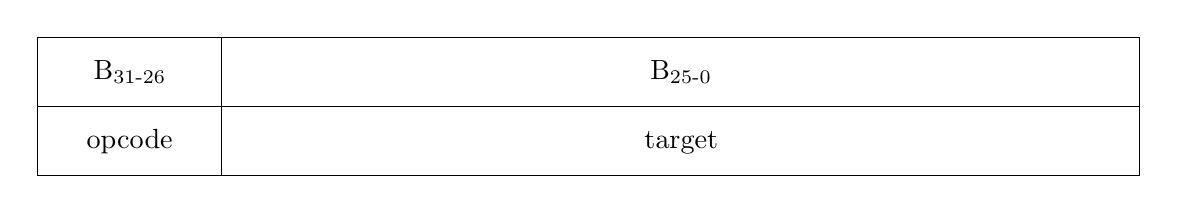
\begin{tikzpicture}[auto,
    every node/.style={rectangle, minimum height=2.5em, text centered, text width=6em, text height=1.5ex, text depth=.25ex},
    field/.style={draw}]
\matrix (m) [ampersand replacement=\&, column sep=-\pgflinewidth, row sep=-\pgflinewidth]
{
\node [field] {$\textrm{B}_{31\textrm{-}26}$}; \&
\node [field, text width=32.5 em] {$\textrm{B}_{25\textrm{-}0}$}; \&
\\
\node [field] {opcode}; \&
\node [field, text width=32.5 em] {target}; \&
\\
};
\end{tikzpicture}
%
  }
  \caption{The bitfields of an J-type format instruction}
  \label{fig:j-type-format-bit-fields}
\end{figure}

For an example the instruction \tt{j} is J-type instruction, and in
its mnemonic form as follows,

\begin{lstlisting}[style=mips_lst]
j target
\end{lstlisting}
%$

\tt{j} is the archetypal jump instruction. In ~\autoref{lst:jump}
``\PC{}'' stands for ``program counter''. The program counter stores
the current address of the instruction that is \emph{currently}
being executed.

In effect, what the \tt{j} instruction does, as shown in
~\autoref{lst:jump}, is re-assign the \PC{} the 32-bit address given
by the upper 4 bits of the \PC{} followed by the 26-bits making up the
target, followed by two zeroes.

\begin{lstlisting}[style=semantics_lst, label={lst:jump}]
PC := PC$_{31\textrm{-}28}$ IR$_{25\textrm{-}0}$ 00
\end{lstlisting}


\subsubsection{MIPS Register Naming and Usage Convention}

Within the MIPS32 architecture there are 32 general-purpose registers,
see \autoref{table:mips-register-naming-and-usage-convention}. The
registers when written out, are preceded by a ``\tt{\$}''.  We use
two formats for addressing a particular register, e.g. \tt{\$0}
through \tt{\$31}. Or, using their equivalent mnemonic
representations, for instance \tt{\$t1}. Both formats may be used
interchangeably in the assembly language.

\begin{table}[H]
\centering
\begin{tabular}{lll}
\toprule
Mnemonic & Register Number & Usage                                                     \\
\midrule
\tt{\$zero}                & 0       & constant 0                                      \\
\tt{\$at}                  & 1       & reserved for assembler                          \\
\tt{\$v0} - \tt{\$v1}      & 2 - 3   & expression evaluation and results of a function \\
\tt{\$a0} - \tt{\$a3}      & 4 - 7   & argument 1 through 4                            \\
\tt{\$t0} - \tt{\$t7}      & 8 - 15  & temporary (not preserved across call)           \\
\tt{\$s0} - \tt{\$s7}      & 16 - 23 & saved temporary (preserved across call          \\
\tt{\$t8} - \tt{\$t9}      & 24 - 25 & temporary (not preserved across call)           \\
\tt{\$k0} - \tt{\$k1}      & 26 - 27 & reserved for OS kernel                          \\
\tt{\$gp}                  & 28      & pointer to global area                          \\
\tt{\$sp}                  & 29      & stack pointer                                   \\
\tt{\$fp}                  & 30      & frame pointer                                   \\
\tt{\$ra}                  & 31      & return address (used by function call)          \\
\bottomrule
\end{tabular}
\caption{MIPS register naming and usage convention}
\label{table:mips-register-naming-and-usage-convention}
\end{table}

\subsection{Instruction Encoding}

In the MIPS32 architecture, all machine instructions are represented
as 32-bit numbers. Throughout this document we will intermittently
dissect these 32-bits into various lengths. We regard the ``upper''
--- or equivalently the ``leftmost'' --- bits as the most significant
bits. Hence, we consider the bit order to be little endian.

In little endian bit notation we denote bit 0 as being the least
significant bit (LSB) and bit 31 as the most significant bit (MSB).

Then, for all MIPS32 instructions we have that the leftmost six bits,
31-26, forms the primary opcode. These bits constitute a field which
are referred to as the \tt{op} field of the instruction.
Depending on the value of the primary opcode there can be an extended
opcode in the rightmost six bits, i.e. bits 0 through 5.  These bits
are referred to as the \funct{} field.\footnote{The decoding of
  the \funct{} field provides details of the required operation
  to the \tt{ALU}.}

Ostensibly, the different fields a MIPS instruction should be divided
into is determined solely by the opcode. The manner in which the bits
are divvied up into fields depends on which instruction format that
the instruction has.

Regardless of the type of the instruction we have that the
\opcode{} field is the uppermost six bits of all MIPS
instructions. Opcode, short for ``operation code'', either identifies
a unique instruction or a \emph{set} of instructions.

While MIPS consists of over a 100 different instructions only 6 bits
are used for the \opcode{}, meaning that the
\opcode{}-field can only be used to differentiate between
$2^6=64$ instructions. 

For R-type instructions an additional 6 bits are used (\textbf{B5-0})
called the ``function'', which serves as a secondary opcode to
identify the instruction. I.e. the tuple

\begin{equation*}
(\opcode{},\ \funct{})
\end{equation*}

is sufficient to \emph{uniquely} identify an R-type instruction.

Other instructions, such as \texttt{bltzal}\footnote{Not an R-type
instruction}, is identified by the tuple

\begin{equation*}
(\opcode{}=1,\ \rt{}=16) \textrm{\hspace{1em}(Remark: base 10)}
\end{equation*}

The MIPS ISA groups its instructions into three
categories:\footnote{Some people consider floating-point and branching
  instructions to be their own respective categories} R-type, I-type, and J-type.

\subsubsection{R-type format}

R-type instructions refer to \emph{register} type instructions. These,
when encoded in machine code, are split into 6 fields of lengths 6, 5,
5, 5, 5, 6 respectively, see ~\autoref{fig:r-type-format-bit-fields}.

\begin{figure}[H]
  % Center the image on the page using makebox  
  \makebox[\textwidth][c]{
    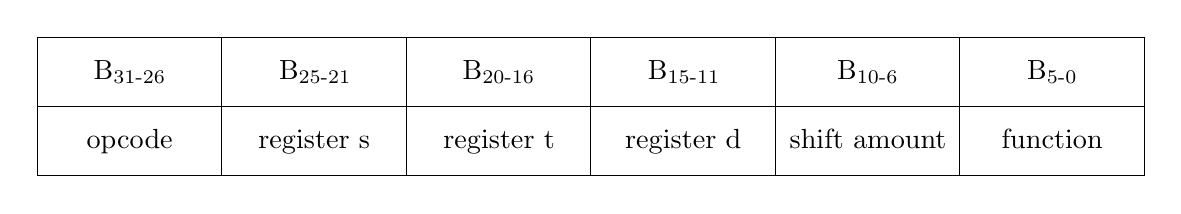
\begin{tikzpicture}[auto,
    every node/.style={rectangle, minimum height=2.5em, text centered, text width=6em, text height=1.5ex, text depth=.25ex},
    field/.style={draw}]
\matrix (m) [ampersand replacement=\&, column sep=-\pgflinewidth, row sep=-\pgflinewidth]
{
\node [field] {$\textrm{B}_{31\textrm{-}26}$}; \&
\node [field] {$\textrm{B}_{25\textrm{-}21}$}; \&
\node [field] {$\textrm{B}_{20\textrm{-}16}$}; \&
\node [field] {$\textrm{B}_{15\textrm{-}11}$}; \&
\node [field] {$\textrm{B}_{10\textrm{-}6}$}; \&
\node [field] {$\textrm{B}_{5\textrm{-}0}$}; \&
\\
\node [field] {opcode}; \&
\node [field] {register s}; \&
\node [field] {register t}; \&
\node [field] {register d}; \&
\node [field] {shift amount}; \&
\node [field] {function}; \&
\\
};
\end{tikzpicture}
%
  } 
  \caption{The bitfields of an R-type format instruction}
  \label{fig:r-type-format-bit-fields}
\end{figure}

For instance, \tt{add} is an R-type instruction, and in
its mnemonic form it looks like

\begin{lstlisting}[style=mips_lst]
add $rd, $rs, $rt
\end{lstlisting}
%$

where \tt{\$rd} refers to some register \tt{d}.

The semantics of the instruction is

\begin{lstlisting}[style=semantics_lst]
R[d] = R[s] + R[t]
\end{lstlisting}

where the addition is signed addition. Hence, \tt{\$rd} is the
target/destination register while the operands \tt{\$rs} and
\tt{\$rt} are the two source registers.\footnote{Notice that the
  mnemonic representation specifies the destination register
  \emph{first} followed by the two source registers but the the actual
  binary format stores the two source registers first, then the
  destination register.}

Certain R-type instructions places certain constraints on its
constituent fields beyond the value of the opcode and the funct
field. Several instructions are only valid if \shamt{} is set to
0, and specifies the shift amount used by shifting instructions such
as \tt{sll} (shift left logical). \tt{clo} (count leading
zeroes) expects both \shamt{} and \tt{rt} to be equal to
zero, and meanwhile \tt{div} (divide with overflow) expects
\rd{} and \shamt{} to be zero.

\subsubsection{I-type format}

I-type stands for "immediate type", and it is decomposed into four
fields. See ~\autoref{fig:i-type-format-bit-fields}.

\begin{figure}[H]
  \makebox[\textwidth][c]{
    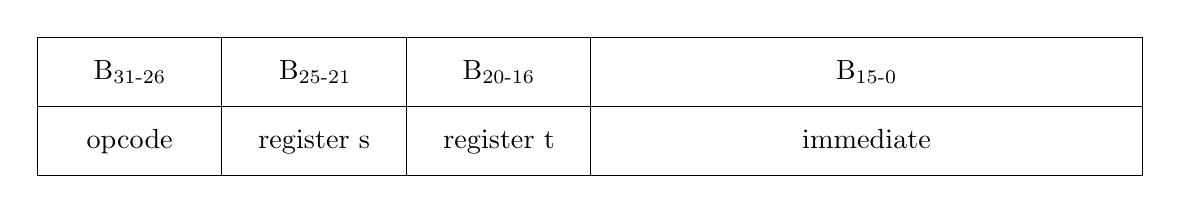
\begin{tikzpicture}[auto,
    every node/.style={rectangle, minimum height=2.5em, text centered, text width=6em, text height=1.5ex, text depth=.25ex},
    field/.style={draw, anchor=west}]
\matrix (m) [ampersand replacement=\&, column sep=-\pgflinewidth, row sep=-\pgflinewidth]
{
\node [field] {$\textrm{B}_{31\textrm{-}26}$}; \&
\node [field] {$\textrm{B}_{25\textrm{-}21}$}; \&
\node [field] {$\textrm{B}_{20\textrm{-}16}$}; \&
\node [field, text width=19.25em] {$\textrm{B}_{15\textrm{-}0}$}; \&
\\
\node [field] {opcode}; \&
\node [field] {register s}; \&
\node [field] {register t}; \&
\node [field, text width=19.25em] {immediate}; \&
\\
};
\end{tikzpicture}
%
  }
  \caption{The bitfields of an I-type format instruction}
  \label{fig:i-type-format-bit-fields}
\end{figure}

The prototypical I-type instruction in its mnemonic form looks as follows,

\begin{lstlisting}[style=mips_lst]
addi $rt, $rs, immed
\end{lstlisting}

In this case, \tt{\$rt} is the destination register, and
\tt{\$rs} is the \emph{only} source register.

The semantics of the \tt{addi} instruction is

\begin{lstlisting}[style=semantics_lst]
R[t] = R[s] + (IR$_{15})^{16}$ IR$_{15\textrm{-}0}$
\end{lstlisting}

where \tt{IR} refers to the instruction register, the register
where the current instruction is stored. \tt{(IR$_{15}$)$^{16}$}
means that bit \textbf{B15} of the instruction register (which is the
sign bit of the immediate value) is repeated 16 times. This is then
followed by \tt{IR$_{15\textrm{-}0}$}, which is the 16 bits of
the immediate value.

Basically, the semantics says to sign-extend the immediate value to 32
bits, add it (using signed addition) to register \tt{R[s]}, and store
the result in register \tt{\$rt}.

For an example,

\begin{lstlisting}[style=mips_lst]
addi $s1, $s2, 100
\end{lstlisting}
%$

stores the value of $(\tt{\$s2} + 100)$ in \tt{\$s1}.

\subsubsection{J-type format}

All jump instructions belong to the J-type format

J-type instructions refer to \emph{jump} type instructions. These,
when encoded in machine code, are split into 2 fields of lengths 6 and
26, respectively. See ~\autoref{fig:r-type-format-bit-fields}.

\begin{figure}[H]
  \makebox[\textwidth][c]{
    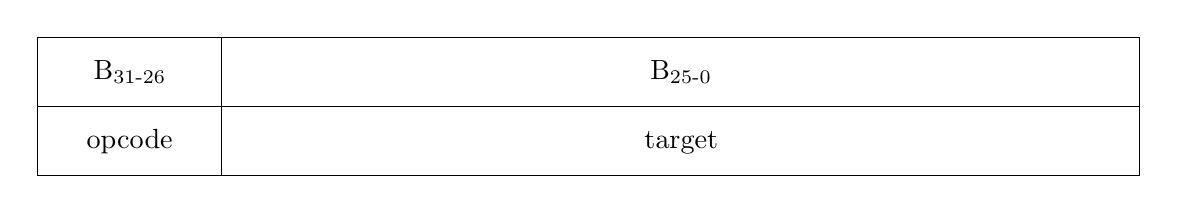
\begin{tikzpicture}[auto,
    every node/.style={rectangle, minimum height=2.5em, text centered, text width=6em, text height=1.5ex, text depth=.25ex},
    field/.style={draw}]
\matrix (m) [ampersand replacement=\&, column sep=-\pgflinewidth, row sep=-\pgflinewidth]
{
\node [field] {$\textrm{B}_{31\textrm{-}26}$}; \&
\node [field, text width=32.5 em] {$\textrm{B}_{25\textrm{-}0}$}; \&
\\
\node [field] {opcode}; \&
\node [field, text width=32.5 em] {target}; \&
\\
};
\end{tikzpicture}
%
  }
  \caption{The bitfields of an J-type format instruction}
  \label{fig:j-type-format-bit-fields}
\end{figure}

For an example the instruction \tt{j} is J-type instruction, and in
its mnemonic form as follows,

\begin{lstlisting}[style=mips_lst]
j target
\end{lstlisting}
%$

\tt{j} is the archetypal jump instruction. In ~\autoref{lst:jump}
``\PC{}'' stands for ``program counter''. The program counter stores
the current address of the instruction that is \emph{currently}
being executed.

In effect, what the \tt{j} instruction does, as shown in
~\autoref{lst:jump}, is re-assign the \PC{} the 32-bit address given
by the upper 4 bits of the \PC{} followed by the 26-bits making up the
target, followed by two zeroes.

\begin{lstlisting}[style=semantics_lst, label={lst:jump}]
PC := PC$_{31\textrm{-}28}$ IR$_{25\textrm{-}0}$ 00
\end{lstlisting}


\subsubsection{Example: Numeric decoding}

Consider the machine-language MIPS32 instruction \tt{0x71014802}.
Depending on the format of the instruction it decomposes into fields
varying lengths.

Recall that for all numbers in the MIPS32 instruction set the leftmost
six bits always represent the opcode for the instruction. The opcode
alone is not always sufficient to identify the particular instruction,
\emph{but} it is always sufficient to identify the format of the
instruction.

The leftmost six bits of \tt{0x71014802} is \tt{0x1c}. It is
\emph{known} that this number corresponds to a set of instructions in
the R-type format. The format specifies into which fields the 32-bit
decomposes into. The number of bits composing each respective field is
given in the bottom row of ~\autoref{fig:r-decomposed},

\begin{figure}[H]
\centering
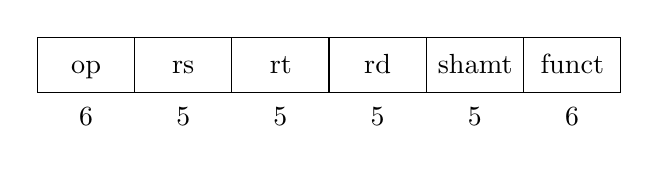
\begin{tikzpicture}[node distance=1em]

\matrix (decomposed-representation) [
  matrix of nodes,
  row sep=0.2em,
  column sep=-\pgflinewidth,
  row 1/.style={
    nodes={
      rectangle, 
      draw, 
      text centered,
          text width=10mm,
      anchor=base,
      text height=.8em,text depth=.2em,minimum size=7mm
    }
  }
] {
op & rs & rt & rd & shamt & funct \\
6 & 5 & 5 & 5 & 5 & 6 \\
};
\end{tikzpicture}

\caption{The length of each respective field for R-type format instructions}
\label{fig:r-decomposed}
\end{figure}

Decomposing \tt{0x71014802} into the fields shown in
\autoref{fig:r-decomposed} yields \tt{rs=8}, \tt{rt=1}, \tt{rd=9},
\tt{shamt=0}, and \tt{funct=2}. The \emph{decomposed representation}
of this instruction in hexadecimal form is thus \tt{[0x1c 8 1 9 0
  2]}.\footnote{The corresponding \emph{decimal representation} is
  \tt{[28 8 1 9 0 2]}}

To identify the particular instruction represented by \tt{0x71014802}
the \funct{} field must be consulted. Pairing the opcode, \tt{0x1c}
and the value in the \funct{} field uniquely identifies the
instruction a \tt{mul} instruction; see \autoref{fig:mul-decomposed}.

\begin{figure}[H]
  \centering
  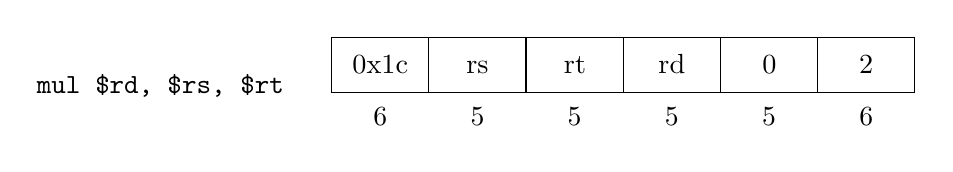
\begin{tikzpicture}[node distance=1em]
\matrix (decomposed-representation) [
  matrix of nodes,
  row sep=0.2em,
  column sep=-\pgflinewidth,
  row 1/.style={
    nodes={
      rectangle, 
      draw, 
      text centered,
          text width=10mm,
      anchor=base,
      text height=.8em,text depth=.2em,minimum size=7mm
    }
  }
] {
0x1c & rs & rt & rd & 0 & 2 \\
6 & 5 & 5 & 5 & 5 & 6 \\
};
\node [left=of decomposed-representation] (mnemonic-representation) {\texttt{mul \$rd, \$rs, \$rt}};
\end{tikzpicture}

  \caption{Decomposition and mnemonic representation of \tt{mul}}
  \label{fig:mul-decomposed}
\end{figure}

Earlier we determined the fields \tt{rs}, \tt{rt} and \rd{} to have
the addresses 8, 1, and 9, respectively. In MIPS registers are named,
following the convention shown in
\autoref{table:mips-register-naming-and-usage-convention}

Replacing the numerical values of \tt{rs}, \tt{rt} and \rd{}, with
their named counterparts yields the \emph{mnemonic representation} of
the instruction to be

\begin{lstlisting}[style=mips_lst]
mul $t1, $t0, $at
\end{lstlisting}
%$

\subsubsection{Example: Mnemonic decoding}

The reverse operation, translating from a human-legible form to the
numerical form, is trivial. Given, of course, that you know the format
that the mnemonic form is in and any conditions pertaining to the
particular instruction. 

Take for instance \tt{div \$t2, \$t4}, given that we know its mnemonic
representation to be on the form

\begin{lstlisting}[style=mips_lst]
div $rs, $rt
\end{lstlisting}
%$

and that due to its nature both \shamt{} and \rd{} is both zero,
together with the fact that we know its opcode and \funct{}, trivially
we substitute all those values in together with the register
addresses. Together we get

\begin{figure}[H]
  \makebox[\textwidth][c]{
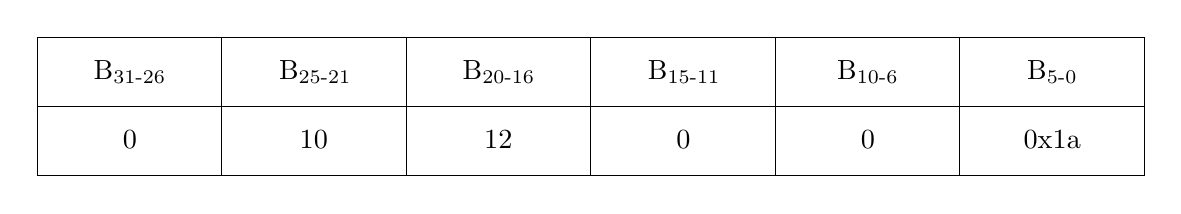
\begin{tikzpicture}[auto,
    every node/.style={rectangle, minimum height=2.5em, text centered, text width=6em, text height=1.5ex, text depth=.25ex},
    field/.style={draw}]
\matrix (m) [ampersand replacement=\&, column sep=-\pgflinewidth, row sep=-\pgflinewidth]
{
\node [field] {$\textrm{B}_{31\textrm{-}26}$}; \&
\node [field] {$\textrm{B}_{25\textrm{-}21}$}; \&
\node [field] {$\textrm{B}_{20\textrm{-}16}$}; \&
\node [field] {$\textrm{B}_{15\textrm{-}11}$}; \&
\node [field] {$\textrm{B}_{10\textrm{-}6}$}; \&
\node [field] {$\textrm{B}_{5\textrm{-}0}$}; \&
\\
\node [field] {0}; \&
\node [field] {10}; \&
\node [field] {12}; \&
\node [field] {0}; \&
\node [field] {0}; \&
\node [field] {0x1a}; \&
\\
};
\end{tikzpicture}
  }
\end{figure}

and the final translation step, and the resulting numerical
representation, is given by a sequence of bit-shift operations, in
this case the following will serve,\footnote{No operations are
  required for the zeroes.}\footnote{Notice that the shift amount (21,
  16) corresponds directly to the lower most bit of the respective fields (rs, rt)}

\begin{lstlisting}
(10 << 21) | (12 << 16) | 0x1a
\end{lstlisting}

which is equal to \tt{0x014c001a}.



\section{Usage and compilation}

We will now describe how to compile and use the supplied software, so
that you may experiment with it later when the solution is described.

The source code may be downloaded at the following two addresses,

\begin{center}
\url{https://github.com/leksak/kilobyte.git} \\
\url{git@github.com:leksak/kilobyte.git}
\end{center}

Or viewed in the following folder
\tt{\raise.17ex\hbox{$\scriptstyle\mathtt{\sim}$}filip/edu/kilobyte}
on the institution's network.

For the duration of this report the directory created by cloning
the repository is referred to as the \emph{root directory}.

\section{Compilation and usage}

In this section the compilation of the software is described as
is the usage of the software

\subsection{Compilation}

Navigate to the root directory of the project.

Whilst there execute the following command to compile the program:

\begin{lstlisting}[style=plain]
$ ./gradlew fatJar
\end{lstlisting}

In the \tt{build/libs} directory you will now find a file named
\tt{kilobyte-all-1.0-SNAPSHOT.jar} which you can run using \tt{java -jar
  kilobyte-all-1.0-SNAPSHOT.jar} given that you have Java 8 shown when running
\tt{java -version}.

\subsubsection{Compiling and running tests}

Navigate to the root directory and hilst there execute the following
command to compile and run the tests:

\begin{lstlisting}[style=plain]
$ ./gradlew test
\end{lstlisting}

In Figure.~\ref{fig:tests} the output yielded by the tests is shown.

\begin{figure}[htpb]
\begin{lstlisting}[style=plain]
$ ./gradlew test             
  [...removed output...]
Test run finished after 1163 ms
[        14 containers found      ]
[         0 containers skipped    ]
[        14 containers started    ]
[         0 containers aborted    ]
[        14 containers successful ]
[         0 containers failed     ]
[        61 tests found           ]
[         1 tests skipped         ]
[        60 tests started         ]
[         0 tests aborted         ]
[        60 tests successful      ]
[         0 tests failed          ]
\end{lstlisting}
\caption{Test results}
\label{fig:tests}
\end{figure}

\subsection{Usage}

The program allows us multiple means of interaction which are listed
when the program is passed the "-h" or "--help" flag which outputs the following
The program supplies two means of interfacing with it, by calling
the program with 0 arguments or the \tt{-h} flag we can get the
user guide supplied with the software

\begin{lstlisting}[style=plain]
$ java -jar build/libs/kilobyte-all-1.0-SNAPSHOT.jar -h
usage: CommandLineDecompiler[OPTION] [file|number]...
    --examples       prints an example for each supported instructions.
 -h,--help           print this message
 -n,--number <arg>   disassemble 32-bit word(s) from stdin
 -S,--suppress       suppress the table header
    --supported      prints all supported instructions
If no argument is given then numbers are read from stdin
\end{lstlisting}

\subsubsection{Decompiling source code from files}

The default setting is that the software interprets its given input
arguments as a filenames, relative to the directory from which you
execute the \tt{.jar} file. In the root directory of the project three
example files are included.

\tt{sample-program.hex} showcases the tabulated output for several
instructions, as well as how error messages for partially legal
instructions are written out.

\tt{sample-decimal.hex} showcases that the program is capable
of handling instructions in base 10. 

\tt{sample-mingled-bases.hex} demonstrates that the program does not
expect the file to be written consistently in either base 10 or base
16 but evaluates this on a per-line basis. A number is interpreted to
be in base 16 if it is prefixed by \tt{0x}. Between the two numbers
a blank-line appears to showcase that the decompiler is robust
enough to ignore such lines.

We can inspect the contents of these files using \tt{cat}
as shown in Listing.~\ref{listing:sample-input-files}.

\begin{figure}
\begin{lstlisting}[style=plain,
    caption=Sample input files,
    label=listing:sample-input-files]
$ cat sample-decimal.hex 
599654392

$ cat sample-mingled.hex
599654392

0xafbf0004

$ cat sample-program.hex
0x23bdfff8
0xafbf0004
0xafa40000
0x28880001
0x11000003
0x20020001
0x23bd0008
0x03e00008
0x2084ffff
0x0c100000
0x8fa40000
0x8fbf0004
0x23bd0008
0x70821002
0x03e00008
0x00012122
\end{lstlisting}
\end{figure}

Similarly we may observe the output of our decompiler in
Listing.~\ref{listing:tabularized-output}, where the
files are passed as a series of arguments.

\subsubsection{Decompiling input numbers}

Additionally, the software provides a secondary means of use, through
the \tt{-n} flag which stands for \emph{number} so that the argument
immediately following the flag.

Notice in Listing.~\ref{listing:parsing-numbers-from-input-arguments}
that it does not matter whether or not the number is in base 10 or
base 16 (as long as numbers in base 16 are prefixed by \tt{0x}).

Lastly, note that the software handles partially valid instructions,
i.e. instructions that may be correctly identified but validates some
condition. For instance, the number \tt{0x00012122} corresponds to the
\tt{sub} instruction. The number decomposes into bitfields according
to the format of the instruction (viz. the R-format), and the opcode
and funct field hold the correct values to identify the instruction as
a \tt{sub} instruction \emph{but} the \tt{shamt} field is not set to
4, which it has to be according to the instruction specification.

When an instruction is partially legal the violating fields are outputted
on the following line, see Listing.~\ref{listing:partially-valid-instructions}.


\begin{landscape}
\section{Listings}

\begin{lstlisting}[style=plain,
    basicstyle=\footnotesize,
    caption=Tabularized output,
    label=listing:tabularized-output,
][htpb]
java -jar build/libs/kilobyte-all-1.0-SNAPSHOT.jar sample-program.hex sample-mingled-bases.hex sample-decimal.hex
Machine Code  |  Format  |  Decomposition     |  Decomposition hexadecimal  |  Source                    |  Errors
0x23bdfff8    |  I       |  [8 29 29 65528]   |  [8 0x1d 0x1d 0xfff8]       |  addi $sp, $sp, 65528      |  
0xafbf0004    |  I       |  [43 29 31 4]      |  [0x2b 0x1d 0x1f 4]         |  sw $ra, 4($sp)            |  
0xafa40000    |  I       |  [43 29 4 0]       |  [0x2b 0x1d 4 0]            |  sw $a0, 0($sp)            |  
0x28880001    |  I       |  [10 4 8 1]        |  [0xa 4 8 1]                |  slti $t0, $a0, 1          |  
0x11000003    |  I       |  [4 8 0 3]         |  [4 8 0 3]                  |  beq $t0, $zero, 3         |  
0x20020001    |  I       |  [8 0 2 1]         |  [8 0 2 1]                  |  addi $v0, $zero, 1        |  
0x23bd0008    |  I       |  [8 29 29 8]       |  [8 0x1d 0x1d 8]            |  addi $sp, $sp, 8          |  
0x03e00008    |  R       |  [0 31 0 0 0 8]    |  [0 0x1f 0 0 0 8]           |  jr $ra                    |  
0x2084ffff    |  I       |  [8 4 4 65535]     |  [8 4 4 0xffff]             |  addi $a0, $a0, 65535      |  
0x0c100000    |  J       |  [3 0]             |  [3 0]                      |  jal 1048576               |  
0x8fa40000    |  I       |  [35 29 4 0]       |  [0x23 0x1d 4 0]            |  lw $a0, 0($sp)            |  
0x8fbf0004    |  I       |  [35 29 31 4]      |  [0x23 0x1d 0x1f 4]         |  lw $ra, 4($sp)            |  
0x23bd0008    |  I       |  [8 29 29 8]       |  [8 0x1d 0x1d 8]            |  addi $sp, $sp, 8          |  
0x70821002    |  R       |  [28 4 2 2 0 2]    |  [0x1c 4 2 2 0 2]           |  mul $v0, $a0, $v0         |  
0x03e00008    |  R       |  [0 31 0 0 0 8]    |  [0 0x1f 0 0 0 8]           |  jr $ra                    |  
0x00012122    |  R       |  [0 0 1 4 4 34]    |  [0 0 1 4 4 0x22]           |  sub $a0, $zero, $at       |   error(s)=["Expected shamt to be zero. Got 4"]
0x23bdfff8    |  I       |  [8 29 29 65528]   |  [8 0x1d 0x1d 0xfff8]       |  addi $sp, $sp, 65528      |  
0xafbf0004    |  I       |  [43 29 31 4]      |  [0x2b 0x1d 0x1f 4]         |  sw $ra, 4($sp)            |  
0x23bdfff8    |  I       |  [8 29 29 65528]   |  [8 0x1d 0x1d 0xfff8]       |  addi $sp, $sp, 65528      | 
\end{lstlisting}

\begin{figure}
\begin{lstlisting}[style=plain,
    basicstyle=\small,
    caption=Parsing numbers from input arguments using the \tt{-n} flag,
    label=listing:parsing-numbers-from-input-arguments]
$ java -jar build/libs/kilobyte-all-1.0-SNAPSHOT.jar -n 599654392 -n 0xafbf0004 --suppress
0x23bdfff8    |  I       |  [8 29 29 65528]   |  [8 0x1d 0x1d 0xfff8]       |  addi $sp, $sp, 65528      |  
0xafbf0004    |  I       |  [43 29 31 4]      |  [0x2b 0x1d 0x1f 4]         |  sw $ra, 4($sp)            |
\end{lstlisting}
\end{figure}

\begin{lstlisting}[basicstyle=\small,
    style=plain,
    caption=Error print-outs for partially valid instructions,
    label=listing:partially-valid-instructions,
  backgroundcolor=\color{mintedbackground}]
$  java -jar build/libs/kilobyte-all-1.0-SNAPSHOT.jar -n 0x00012122 --suppress
0x00012122    |  R       |  [0 0 1 4 4 34]    |  [0 0 1 4 4 0x22]           |  sub $a0, $zero, $at       |   error(s)=["Expected shamt to be zero. Got 4"]
\end{lstlisting}
\end{landscape}


\begin{appendix}


\section{Kotlin}

Kotlin is a statically-typed programming language that runs on the
Java Virtual Machine (JVM). While not syntax compatible with Java,
Kotlin is designed to interoperate with Java code and is reliant on
Java code from the existing Java Class Library, such as the
collections framework.

\subsection{Why Kotlin}

Kotlin compiles to JVM bytecode (or JavaScript, but that is not
pertinent to this project). It solves problems commonly associated
with Java, in particular it requires far less boiler-plate to the
benefit of legibility without incurring a refactor-ability
cost.\footnote{Project Lombok can also offset a lot of Java
  boiler-plate, and it is a ``plain'' Java library}

Additionally its type system helps us avoid null-pointer exceptions
while still retaining a notion of null which is useful when working
with APIs that do (Java).

It does this by making a distinction between nullable and non-nullable
datatypes. All nullable objects must be declared with a ``\tt{?}''
postfix after the type name. Operations on nullable objects need
special care from developers; a null-check must be performed before
using the value. Kotlin provides special operators for this.

\subsubsection{Sum types}

% TODO: Should we continue using io.atlassian.fugue.Either or go for
% a sum type with valid and partially valid instruction

\subsubsection{Singletons and class-less functions}

Want a singleton? Create an object:

object ThisIsASingleton {
    val companyName: String = "JetBrains"
  }

  \subsubsection{Named arguments}



\subsection{Kotlin --- applied}

\begin{lstlisting}[style=java]
@JvmField val ADD = Instruction(
      iname = "add",
      opcode = 0,
      funct = 0x20,
      mnemonicRepresentation = "add \$t1, \$t2, \$t3",
      numericRepresentation = 0x014b4820,
      description = "Addition with overflow,. Put the" +
            " sum of registers rs and rt into register" +
            " rd. Is only valid if shamt is 0.",
      format = Format.R,
      pattern = ParametrizedInstructionRoutine.INAME_RD_RS_RT)
\end{lstlisting}



\clearpage

\section{List of supported instructions}

The decompiler has support for all of the following instructions,

\begin{multicols}{4}
\begin{itemize}
\item add
\item addu
\item addi
\item addiu
\item and
\item andi
\item clo
\item clz
\item div
\item divu
\item mult
\item multu
\item mul
\item madd
\item maddu
\item msub
\item msubu
\item nor
\item or
\item ori
\item sll
\item sllv
\item sra
\item srav
\item srl
\item srlv
\item sub
\item subu
\item xor
\item xori
\item lui
\item slt
\item sltu
\item slti
\item sltiu
\item beq
\item beql
\item bgez
\item bgezl
\item bgezal
\item bgczall
\item bgtz
\item bgtzl
\item blez
\item bltzal
\item bltzall
\item bltz
\item bltzl
\item bne
\item bnel
\item j
\item jal
\item jalr
\item jr
\item teq
\item teqi
\item tne
\item tnei
\item tge
\item tgeu
\item tgei
\item tgeiu
\item tlt
\item tltu
\item tlti
\item tltiu
\item nop
\item blezl
\item lb
\item lbu
\item lh
\item lhu
\item lw
\item lwc1
\item lwc2
\item lwl
\item lwr
\item ll
\item sb
\item sh
\item sw
\item swc1
\item swc2
\item sdc1
\item sdc2
\item swl
\item sc
\item mfhi
\item mflo
\item mthi
\item mtlo
\item movn
\item movz
\item pref
\item ldc1
\item ldc2
\end{itemize}
\end{multicols}
\end{appendix}

\section{Example decompilations}

Here we present a sample decompilation for each of the instructions
listed in the previous section.

\lstMakeShortInline=

	\begin{tabular}{lcl}
      \toprule
      Hex & & Mnemonic \\
      \midrule
\tt{0x14b4820}	& $\longrightarrow$		& =add $t1, $t2, $t3= \\
\tt{0x14b4821}	& $\longrightarrow$		& =addu $t1, $t2, $t3= \\
\tt{0x21490004}	& $\longrightarrow$		& =addi $t1, $10, 4= \\
\tt{0x25490004}	& $\longrightarrow$		& =addiu $t1, $t2, 4= \\
\tt{0x14b4824}	& $\longrightarrow$		& =and $t1, $t2, $t3= \\
\tt{0x31490004}	& $\longrightarrow$		& =andi $t1, $t2, 4= \\
\tt{0x71404821}	& $\longrightarrow$		& =clo $t1, $t2= \\
\tt{0x71404820}	& $\longrightarrow$		& =clz $t1, $t2= \\
\tt{0x12a001a}	& $\longrightarrow$		& =div $t1, $t2= \\
\tt{0x12a001b}	& $\longrightarrow$		& =divu $t1, $t2= \\
\tt{0x12a0018}	& $\longrightarrow$		& =mult $t1, $t2= \\
\tt{0x12a0019}	& $\longrightarrow$		& =multu $t1, $t2= \\
\tt{0x70821002}	& $\longrightarrow$		& =mul $v0, $a0, $v0= \\
\tt{0x712a0000}	& $\longrightarrow$		& =madd $t1, $t2= \\
\tt{0x712a0001}	& $\longrightarrow$		& =maddu $t1, $t2= \\
\tt{0x712a0004}	& $\longrightarrow$		& =msub $t1, $t2= \\
\tt{0x712a0005}	& $\longrightarrow$		& =msubu $t1, $t2= \\
\tt{0x14b4827}	& $\longrightarrow$		& =nor $t1, $t2, $t3= \\
\tt{0x14b4825}	& $\longrightarrow$		& =or $t1, $t2, $t3= \\
\tt{0x35490004}	& $\longrightarrow$		& =ori $t1, $t2, 4= \\
\tt{0x14a4800}	& $\longrightarrow$		& =sll $t1, $t2, $10= \\
\tt{0x14b4804}	& $\longrightarrow$		& =sllv $t1, $t2, $t3= \\
\tt{0x14a4803}	& $\longrightarrow$		& =sra $t1, $t2, $10= \\
\tt{0x14b4807}	& $\longrightarrow$		& =srav $t1, $t2, $t3= \\
\tt{0x14a4802}	& $\longrightarrow$		& =srl $t1, $t2, $10= \\
\tt{0x14b4806}	& $\longrightarrow$		& =srlv $t1, $t2, $t3= \\
\tt{0x14b4822}	& $\longrightarrow$		& =sub $t1, $t2, $t3= \\
\tt{0x14b4823}	& $\longrightarrow$		& =subu $t1, $t2, $t3= \\
\tt{0x14b4826}	& $\longrightarrow$		& =xor $t1, $t2, $t3= \\
\tt{0x39490004}	& $\longrightarrow$		& =xori $t1, $t2, 4= \\
\tt{0x3c090004}	& $\longrightarrow$		& =lui $t1, 4= \\
\tt{0x14b482a}	& $\longrightarrow$		& =slt $t1, $t2, $t3= \\
\tt{0x14b482b}	& $\longrightarrow$		& =sltu $t1, $t2, $t3= \\
\tt{0x29490004}	& $\longrightarrow$		& =slti $t1, $t2, 4= \\
\tt{0x2d490004}	& $\longrightarrow$		& =sltiu $t1, $t2, 4= \\
\tt{0x112a0004}	& $\longrightarrow$		& =beq $t1, $t2, 4= \\
\tt{0x512a0006}	& $\longrightarrow$		& =beql $t1, $t2, 6= \\
\tt{0x5210005}	& $\longrightarrow$		& =bgez $t1, 5= \\
\tt{0x5230005}	& $\longrightarrow$		& =bgezl $t1, 5= \\
\tt{0x531000a}	& $\longrightarrow$		& =bgezal $t1, 10= \\
\tt{0x533000a}	& $\longrightarrow$		& =bgczall $t1, 10= \\
\tt{0x1d200004}	& $\longrightarrow$		& =bgtz $t1, 4= \\
\tt{0x5d200006}	& $\longrightarrow$		& =bgtzl $t1, 6= \\
\tt{0x19200004}	& $\longrightarrow$		& =blez $t1, 4= \\
\tt{0x530000a}	& $\longrightarrow$		& =bltzal $t1, 10= \\
\tt{0x532000a}	& $\longrightarrow$		& =bltzall $t1, 10= \\
\tt{0x5200005}	& $\longrightarrow$		& =bltz $t1, 5= \\
\tt{0x5220005}	& $\longrightarrow$		& =bltzl $t1, 5= \\
\bottomrule 
    \end{tabular}

	\begin{tabular}{lcl}
      \toprule
      Hex & & Mnemonic \\
      \midrule
\tt{0x152a0004}	& $\longrightarrow$		& =bne $t1, $t2, 4= \\
\tt{0x552a0006}	& $\longrightarrow$		& =bnel $t1, $t2, 6= \\      
\tt{0x8000004}	& $\longrightarrow$		& =j 4= \\
\tt{0xc100000}	& $\longrightarrow$		& =jal 0x00400000= \\
\tt{0x1404809}	& $\longrightarrow$		& =jalr $t1, $t2= \\
\tt{0x1200008}	& $\longrightarrow$		& =jr $t1= \\
\tt{0x12a0034}	& $\longrightarrow$		& =teq $t1, $t2= \\
\tt{0x52c0005}	& $\longrightarrow$		& =teqi $t1, 5= \\
\tt{0x12a0036}	& $\longrightarrow$		& =tne $t1, $t2= \\
\tt{0x52e0005}	& $\longrightarrow$		& =tnei $t1, 5= \\
\tt{0x12a0030}	& $\longrightarrow$		& =tge $t1, $t2= \\
\tt{0x12a0031}	& $\longrightarrow$		& =tgeu $t1, $t2= \\
\tt{0x5280005}	& $\longrightarrow$		& =tgei $t1, 5= \\
\tt{0x5290005}	& $\longrightarrow$		& =tgeiu $t1, 5= \\
\tt{0x12a0032}	& $\longrightarrow$		& =tlt $t1, $t2= \\
\tt{0x12a0033}	& $\longrightarrow$		& =tltu $t1, $t2= \\
\tt{0x52a0005}	& $\longrightarrow$		& =tlti $t1, 5= \\
\tt{0x52b0005}	& $\longrightarrow$		& =tltiu $t1, 5= \\
\tt{0x0}	& $\longrightarrow$		& =nop= \\
\tt{0x59200006}	& $\longrightarrow$		& =blezl $t1, 6= \\
\tt{0x81490007}	& $\longrightarrow$		& =lb $t1, 7($t2)= \\
\tt{0x9149000b}	& $\longrightarrow$		& =lbu $t1, 11($t2)= \\
\tt{0x85490008}	& $\longrightarrow$		& =lh $t1, 8($t2)= \\
\tt{0x9549000c}	& $\longrightarrow$		& =lhu $t1, 12($t2)= \\
\tt{0x8d49000a}	& $\longrightarrow$		& =lw $t1, 10($t2)= \\
\tt{0xc7bf0004}	& $\longrightarrow$		& =lwc1 $ra, 4($sp)= \\
\tt{0xcbbf0004}	& $\longrightarrow$		& =lwc2 $ra, 4($sp)= \\
\tt{0x89490009}	& $\longrightarrow$		& =lwl $t1, 9($t2)= \\
\tt{0x9949000d}	& $\longrightarrow$		& =lwr $t1, 13($t2)= \\
\tt{0xc3bf0004}	& $\longrightarrow$		& =ll $ra, 4($sp)= \\
\tt{0xa1490004}	& $\longrightarrow$		& =sb $t1, 4($t2)= \\
\tt{0xa5490004}	& $\longrightarrow$		& =sh $t1, 4($t2)= \\
\tt{0xafbf0004}	& $\longrightarrow$		& =sw $ra, 4($sp)= \\
\tt{0xe7a90004}	& $\longrightarrow$		& =swc1 $t1, 4($sp)= \\
\tt{0xeba90004}	& $\longrightarrow$		& =swc2 $t1, 4($sp)= \\
\tt{0xf7a90004}	& $\longrightarrow$		& =sdc1 $t1, 4($sp)= \\
\tt{0xfba90004}	& $\longrightarrow$		& =sdc2 $t1, 4($sp)= \\
\tt{0xa9490004}	& $\longrightarrow$		& =swl $t1, 4($t2)= \\
\tt{0xe3a90004}	& $\longrightarrow$		& =sc $t1, 4($sp)= \\
\tt{0x4810}	& $\longrightarrow$		& =mfhi $t1= \\
\tt{0x4812}	& $\longrightarrow$		& =mflo $t1= \\
\tt{0x1200011}	& $\longrightarrow$		& =mthi $t1= \\
\tt{0x1200013}	& $\longrightarrow$		& =mtlo $t1= \\
\tt{0x14b480b}	& $\longrightarrow$		& =movn $t1, $t2, $t3= \\
\tt{0x14b480a}	& $\longrightarrow$		& =movz $t1, $t2, $t3= \\
\tt{0xcfa10002}	& $\longrightarrow$		& =pref 1, 2($sp)= \\
\tt{0xd7a90004}	& $\longrightarrow$		& =ldc1 $t1, 4($sp)= \\
\tt{0xdba90004}	& $\longrightarrow$		& =ldc2 $t1, 4($sp)= \\
\bottomrule 
    \end{tabular}

\clearpage

\printbibliography

\end{document}
